

\chapter{Úvod}
V úvode by som Vás rád oboznámil s témou mojej bakalárskej práce Systém monitorovania stavu plánovacích úloh, ktorá bola zverejnená spoločnosťou Red Hat. Tento systém je schopný riešiť rozličné plánovacie problémy, ktoré definovaný vo formáte XML. Plánovacím problémom chápeme rovnako problémy z bežného života(napríklad optimálna cesta pre vozidlá logistickej spoločnosti ), tak aj problémy z hľadiska informačných technológií(napríklad plánovanie testov na serveri). Podmienkou možnosti plánovania je existencia pravidiel a definičných entít pre konkrétny problém. Riešenie je realizovaný frameworkom OptaPlanner, ktorý na základe pravidiel a definičných entít pre danú úlohu sa pokúsi nájsť najlepšie riešenie, ktorý poskytne ako výsledok. Práca obsahuje popis monitorovacie systému, ktorý sa skladá z grafického rozhrania, ktoré zobrazuje stav plánovacích problémov a priebežný stav výpočtu a výpočtovej časti, ktorá rieši plánovacie problémy frameworkom OptaPlanner-om, ktoré medzi sebou komunikujú. Časť realizujúca riešenie je optimalizovaná pre riešenie problému N Dám. Obe časti systému sú založené na Java EE technológiách v kombinácií s rôznymi štýlovacími frameworkami, ktoré zabezpečili prenositeľnosti užívateľského rozhrania na mobilný telefón. Užívateľské rozhranie je sprístupňované na základe role užívateľa a obsah mechanizmy, ktoré zabezpečujú systém pred zneužitím. \newline \indent Rozhranie obecne umožňuje zobrazovať informácie o úlohách, vyhľadávať úlohy podľa určitého kritéria, editovať definície úloh rovnako aj spúšťať/pozastatovať plánovanie úloh. Okrem umožňuje spravovať užívateľov a organizácie, ktoré sú sprístupnené len konkrétnej užívateľskej role. Výsledkom práce je intuitivné rozhranie s rýchlou učiacou sa krivkou, ktoré je otestované širokou škálou užívateľov, ktorý okrem toho vyjadrili svoje osobné pocity z navrhnutého rozhrania a poskytli spätnú väzbu na možné vylepšenia rozhrania. Rozhranie bolo okrem otestované na platforme UNIX prostredníctvom nástroja Arquillian a JUnit so zreteľom na citlivé časti systému. \newline \indent Druhá kapitola sa venuje Java EE platforme a jej technológiám potrebných k vytvoreneniu systému\ref{JavaEE}. Nájdete tu stručné vysvetlenie spojené poprekladané s obrázkami pre lepšiu názornosť. Na záver kapitoly bude uvedená implementácii Java EE technológií open-source kontajnerom JBoss. \newline \indent V tretej kapitole bude vysvetlený systém OptaPlanner počínajúc elementárnymi časťami potrebnými k dotvoreniu celkového obrazu o probléme plánovania\ref{optaplannerC}. Bude bližšie vysvetlený pojem \uv{plánovací problém}, rovnako bude rozobratý 1 konkrétny typ problému s obrázkom pre lepšie pochopenie. V tejto kapitole sa oboznámime s princípom plánovania prostredníctvom tohto frameworku, rovnako ja konfiguráciu toho frameworku. \newline \indent V štvrtej kapitole sa prezentujeme špecifikáciu systému monitorovania, rovnako aj analyzuje použité technológie\ref{impl}. Následne prejdeme ku konkrétnemu návrhu a rozdeleniu systému na jednotlivé časti. V ďalšej časti uvedieme spôsob implementovania a celú kapitolu ukončíme zmienkou a testovaní aplikácie a vyhodnotení. V záverečnej kapitole zhrnenieme obsah celej práce, zhodnotíme jej prínos a možnosť ďalšieho rozšírenia\ref{zaver}.\newline \indent  V sekcii príloh nájdeme postup na inštaláciu a spustenie aplikácie rovnako ako aj kompletný prehľad navrhnutého rozhrania a predloženého dotazníka\ref{priloh}.


\chapter{Java Enterprise edition 6}\label{JavaEE}
\section{Motivácia}
Nasledujúca kapitola poskytuje prehľad o platforme Java EE 6 vrátané technológií, ktoré sú používané pri implementácií systému monitorovania. Kapitola sa zameriava na pochopenie obecného princípu vytvárania aplikácií založených na Java Enterprise Edition(Java EE) platforme. Ďalej prechádza k vysvetlenie konkrétnch technológií Java EE pre tvorbu užívateľského rozhrania, rovnako aj komunikácie medzi časťami systému. Následne sú vysvetlené obecné princípy používaný jazyk Java, na ktorom je postavená platforma Java EE spolu s nástrojmi na implementáciu a testovanie výsledného systému. \newline \indent V závere kapitoly je rozobratý Java EE kontajner JBoss, ktorý je použitý pre nasadeniem beh a spravovanie výsledného systému\ref{jbossc}. Dôvodom použitia jazyka a na nej založenej platforme je použitie Java EE kontajnera, rovnako aj možnosť použitia pokročilých nástrojov na testovanie a nástroja na spravovanie závislosti, ktorý je primárne určený pre jazyk Java. 


\section{Špecifikácia platformy}
Základom Java EE je štandard Java Standard Edition(Java SE). Java EE predstavuje platformu a poskytuje knižnice určené zjednodušenie vývoja komplexných webových a podnikových aplikácií\cite{fitWeb}. Tieto aplikácie sú viacvrstvové z dôvodu lepšej prenositeľnosti, nasaditeľnosti a modifikovateľnosti. Na Java EE môžme nahliadať ako na kolekciu špecifikáciu od Sun/Oracle. Java označuje okrem programovacieho jazyka, tak isto aj platformu. Java platforma sa skladá z virtuálneho stroja a príslušného Application Programming Interface(API). Virtuálny stroj je behové prostredie našej aplikácie zloženého z tried, ktoré bolo preložené do byte kódu. Tento virtuálny stroj býva navrhnutý pre konkrétny operačný systém. API je sada vytvorených tried, ktoré môžme využiť pri implementácií aplikácie a sprístupňuje funkčnosť virtuálneho stroja\cite{javaeespec}.\newline \indent Základom používania Java EE aplikácií je prítomnosť štandardného API využívané enterprise aplikáciami. Java EE teda poskytuje, ktoré usnadňujú vývoj v rôznych oblastiach, či je to oblasť webových služieb(napríklad Java API for XML Web Services), správa transakcií(napríklad Java Transaction API) alebo rôzne iné oblasti. Aplikácia, ktorá pokrýva všetky API, ktoré spĺňajú špecifikáciu Sun/Oracle pre Java EE sa nazýva aplikačný server. Aplikačný server rovnako poskytuje aj klasické služby na jeho spravovanie. Referenčnou implementáciou je server GlassFish. Základom aplikácie sú komponenty, ktoré predstavuju základné jednotky aplikácie, ktoré sa nasadzujú na server. Komponent existuje niekoľko druhou, ale len niektoré sa nasadzujú na aplikačný server. Každý aplikačný server obsahuje kontajnery, ktoré sa starajú o poskynutie funkcionality konkrétnej komponente. Java EE platforma špecifikuje aplikačný model Java EE aplikácie, ktorá je rozdelená do vrstiev podľa fukčnosti.

\section{Aplikačný model}
Java EE definuje aplikácie, ktoré sú viacvrstvové(multitier). Pojmom viacvrstvosť je myslené rozdelenie aplikácie podľa funkčnosti na menšie celky(ktoré nazýva stupne), ktoré majú nastarosť určitú úlohu. Každá vrstva je predstavovaná inými technológiami. Vo výsledku jednotlivé vrstvy medzi sebou komunikujú a toto rozdelenie uľahčuje a zprehľadňuje presnosť vývojové cykly aplikácie. Každá vrstva je reprezentovaná komponenta, ktorá predstavuje funkčnú časť programu zostavenú z tried a súborov, ktorá je vložená do Java EE aplikácie a interaguje s inými komponentami\cite{Pravidla}. Jednotlivé komponenty sa následne rôzne inštalujú na rôzne vrstvy v závislosti od ich príslušnosti(každý stupeň môže byť fyzicky na inom aplikačnom serveri). Jednotlivé stupňe sa skladajú z rôznych komponent, pričom stupne sú rozdelené nasledovne:
\begin{itemize}
\item Klientský stupeň sa skladá z klientských komponenent, ktoré bežia na klientskom počítači
\item Stredná vrstva sa skladá z webových a podnikových komponent, ktoré bežia na Java EE serveri, ktorý predstavuje prostredie pre nasadenie, spravovanie a beh podnikových a webových komponent Java EE aplikácie
\item Najnižšia vrstva predstavuje externé systémy využívané Java EE aplikáciou. Typicky sa jedná o databázový server a externé systémy označujeme názvom \uv{Enterprise Information System(EIS)}
\end{itemize}

Typicky beží medzi klientskom a databázou častou viac-vláknový Java EE server. Na základe tohto rozdelenia môžme uviesť, že platforma Java EE sa používa vývoj vo webovej a podnikovej vrstve, ktoré bežia na Java EE serveri.  Na obrázku č. \ref{model} môžme vidieť viacvrstvové rozdelenie.
\begin{figure}[htb]

\begin{center}

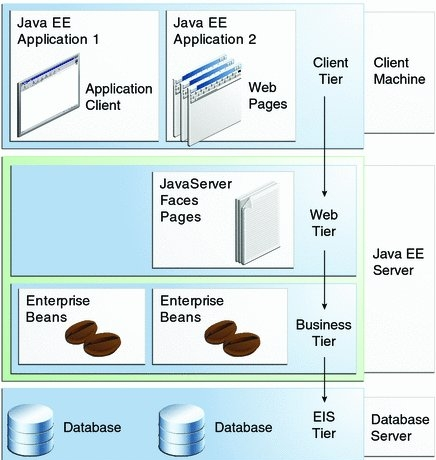
\includegraphics[scale=0.5]{model.jpg} 
\caption{Model Java EE prevzaté z [http://docs.oracle.com/javaee/6/tutorial/doc/]}
\label{model}

\end{center}

\end{figure}
Klient pristupuje k Java EE aplikácií na Java EE serveri z klientskej stanice, prostredníctvom tenkého klienta(webový prehliadačo), ktorý sa nazýva \uv{tenký klient}(pretože sa nedotazuje priamo na databázový server), alebo klientská aplikácia, ktorý sa nazýva \uv{hrubý klient}. Tenký klient pozostáva z:  Webové prehliadača, ktorý zobrazuje stránky a dynamické webové stránkz pozostávajúce  z rôzneho značkovacieho jazyka, ktoré sú generované webovými komponentami. Tenký klient sa dotazuje prostredníctvom Hypertext Transfer protokolu(HTTP), čo je internetový protokol pre výmenu hyperxtových dokumentov, na webové komponenty na Java EE serveri. Hrubý klient, ktorý môže byť reprezentovaný rozličnými Java SE technológiami pre tvorbu užívateľských rozhraní, sa môže priamo dotazovať podnikových komponent a preskočiť tak komunikáciu s webovými komponentami. \newline \indent Stredná vrstva sa delí na webovú vrstvu, ktorá je prezentovaná technológiami JavaServer Faces a JavaServer Pages. Druhá časť strednej vrstvy takzvaná podniková vrstva býva reprezentovaná technológiu EnterpriseJava Beans, ktoré vytvárajú logiku aplikácie. Webová vrstva reprezentovaná je reprezentovaná webovými komponentami, ktoré spracovávajú požiadavky od užívateľa a generujú odpoveď, ktorú posielajú naspäť užívateľovi. Môžu pritom kontaktovať aj podnikové komponenty pre zistenie dodatočných informácií. Podniková vrstva je reprezentovaá podnikovými komponentami, ktoré tvoria základ aplikácie. Tieto komponenty môžu prijímať požiadavky od klienta alebo webovej vrstvy a následne generujú odpovede, pričom môžu komunikovať s najnižšou vrstvou(napríklad komunikovať s databázovým serverom). Táto vrstva beží na Java EE serveri. \newline \indent Najnižšia vrstva predstavuje rozličné externé systémy, ktoré aplikácia môže využívať, či už sa jedná o databázový systém, alebo iné. Vrstva býva označovaná skratkou EIS.



\section{JavaServer Pages}
JavaServer Pages(JSP) technológia je jazyk, ktorý umožňuje priamo vkladanie Java kódu do HyperText Markup Language(HTLM) kódu. HTML je značkovvací jazyk pre vytváranie webových stránok, ktorý obsahuje HTML značky. Pre vloženia java kódu v HTML stránke sa používajú nasledujúce značky: \emph{<\%} \emph{\%>} medzi, ktoré sa vloží príslušný java kód. Takéto časti v HTML stránke sa nazývaju \uv{skriptlety}. Tieto skriplety sú dynamické, to znamená, že sú vykonávané za behu aplikácie. Behom aplikácie je myslené nasadenie jsp stránky(stránka obsahújca skriplety) na Java EE server, ktorý zabezpečuje jeho vykonávanie prostredníctvom volania jsp kontajneru.

\begin{figure}[htb]

\begin{center}

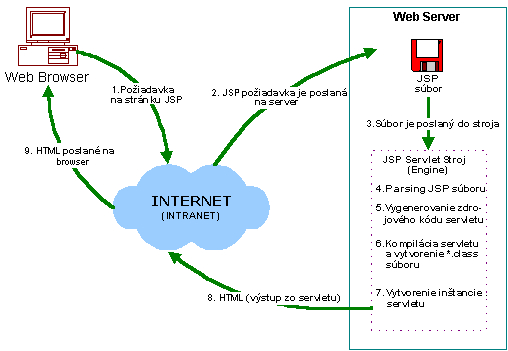
\includegraphics[scale=0.5]{architecture.jpg} 
\caption{JSP architektúra  prevzáte z [http://interval.cz/clanky/javaserver-pages-pro-vsechny/] }
\label{jsp}

\end{center}

\end{figure}
Na nasledujjúcom obrázku č.\ref{jsp} je zobrazený princíp technológie JSP. Základnou časťou je existenia JSP stránky a jej nasadenie na Java EE serveri. V 1.kroku existuje užívateĺ, ktorý je reprezentovaný webovým prehliadačom, ktorý zažiada o JSP stránku. Java EE server prijme požiadavku od klienta a zistí, že sa jedná o požiadavku o JSP stránku . Ten zavolá JSP servlet kontajner na spracovanie žiadosti, ktorý obsahuje JavaServer Pages prekladač, ktorý obsluhuje spracovanie, kontrolu a generovanie. Ten JSP servlet stroj spracováva JSP stránku a vyhodnocuje skriplety a nahradzje ich výsky HTML kódom, ktorý produkuje na výstup. Výstupom zo JSP servletu, ktorý vznikol ako požiadavka o JSP stránku je html stránka, ktorá je predaná užívateľovi, ktorý si ju zobrazí. Výhodou tejto technológie je, že pri žiadosť o JSP stránku je, že pri zmene sa nemení celý obsah stránky ale len jej časť, ktorá bola zmenená. Takže takéto JSP stránky sú dynamické a umožňujú zmenu obsahu za behu.



\subsection{JavaServer Faces}
JavaServer Faces(JSF) je framework pre tvorbu užívateľských rozhraní webových aplikácií, ktoré bežia na Java EE serveri. JSF framework vytvára aplikácie na základe  Model-View-Controller(MVC). MVC predstavuje sotwarovú architektúru, ktorá rozdeľuje aplikáciu na dátový model, užívateľské rozhranie a riadiacu logiku do nezávislých častí. Princíp je nasledujúci:
\begin{itemize}
\item Model - špecifická reprezentácia dát, s ktorými pracuje aplikácia
\item View - prevádza data aplikácie vhodné do podoby prezentácie užívateľa
\item Controller - reaguje na udalosti, typicky od klienta a zabezpečuje zmeny v model alebo view

\end{itemize}
Pri využítí tohto frameworku programátor vkladá predpripravené komponenty(tlačidlá, vyskakovacie okná, rolovacie zoznamy, \ldots) a mapuje ich na príslušné triedy. JSF sa skladá z 2 častí:
\begin{itemize}
\item JSF API - obsahuje komponenty užívateľského rozhrania, umožňuje ich správu, validáciu vstupov, zpracovanie udalostí, navigáciu a iné
\item Knižnica tagov(tag library), ktorá môže byť alternatívne nahradená JSP knižnicou tagov - prostredníctvom týchto špeciálnych tagov vkladáme komponenty užívateľského rozhrania na stránku a upravuje ich chovanie pomocou atribútov alebo mapovaním na triedy. Každá komponenta je definovaná triedou, ktorá určuje jej funkcionalitu. Tagy jednotlivých knižníc sú rozlišované na základe menných priestorov.
\end{itemize}

JSF umožňuje mať výstup v podobe HTML jazyka, alebo iného jazyka v závislosti od definičných tried komponent. Základnou implementáciu prevádza JSF komponenty do HTML kódu.
\subsection{JSF aplikácia}
JSF aplikácia je klasická webová aplikácia, ktorá obsahuje aj svoje špecifiká. Základná štruktúra JSF aplikácie je nasledujúca, pričom nie všetky časti sú povinné:
\begin{itemize}
\item Súbory značkovanie jazyka HTML alebo Extensible Hypertext Markup Language(XHTML)\cite{xhtmlbook}, ktoré obsahuju komponenty užívateľského rozhrania z knižnice tagov, ktoré môžu byť namapované na tzv. \uv{managed bean-y}
\item Managed Beans - java triedy, ktoré sú spravované JSF frameworkom. Najdôležitejšie sú \uv{backing bean}, ktoré zabezpečujú funkcionalitu na HTML/XHTML stránke, udržujú stav komponent, zpracovájú udalosti, validáciu \ldots. Ich konfigurácia sa realizuje v súbore \emph{faces-config.xml}
\item Konfiguračný súbor \emph{faces-config.xml}, v ktorom sa definujú backing beany spolu s ich typom, navigácia, validátory(java triedy, ktorá spracovávajú zadané hodnoty a generujú výstup), \ldots
\item Popisovač nasadenia \emph{web.xml}, ktorý umožňuje nastavenie uvítacích stránok, filtre, servlety a \ldots
\end{itemize}
Neoddeliteľnou súčasťou tohto frameworku je Expression Language(EL), je jazyk, ktorý umožňuje dynamicky pristupovať k metódam javovských tried,(backing bean) rovnako dokáže získať a nastaviť hodnotu danej komponenty.Pri preklade sa vygenerejú závislosti na backing beans. Backing beans dokáže za behu spracovávať údaje zadané na webovú stránku, rovnako dokáže obstarať validáciu vstupov,  následne metódy a vlastnosti, ktoré sú volané alebo sú im predávané údaje z vygenerovavnej stránky(HTML alebo XHTML) do backing bean-y alebo opačne. \newline \indent Obecne Managed Beans môžu byť nasledujúceho typu, pričom typy managed beans sa uvádzajú v súbore faces-config.xml:
\begin{itemize}
\item @RequestScoped Managed beana prežíva pokiaľ  existuje HTTP požiadavok. Vytvára sa pri vytvorený požiadavku a zaniká pri zrušení HTTP požiadavku
\item @NoneScoped Managed Beana existuje tak dlho ako existuje vyhodnotenie Facelets na stránke, po vyhodnotení zaniká
\item @ViewScoped Managed beana prežíva pokiaľ existuje interakcia s danou JSF stránkou. Vytvára sa pri žiadosti o danú stránku a zaniká pokiaľ užívateľ prejde na inú JSF stránku
\item @SessionScoped Managed bean prežíva tak dlho pokiaľ existuje HTTP sedenie. Vytvára sa pri 1.požiadavke o danú stránku a zaniká pri invalidácií daného HTTP sedenia
\item @ApplicationScoped Managed Bean prežíva dokiaľ existuje aplikácia. Je vytvorená pri prvej interakcii s aplikáciou a zaniká pri ukončení aplikácie
\item @CustomScoped Managed Bean existuje dokiaľ existuje záznam o bean-e v v custom Map, ktorá je vytvorená pre existenciu danej beany
\end{itemize}
V poslednom rade treba uviesť životný cyklus JSF aplikácie.

Celý štandardný cyklus cyklus spracovania požiadavky a následne generovania odpovedi je popísaný na nasledujúcom obrázku.
\begin{figure}[htb]

\begin{center}

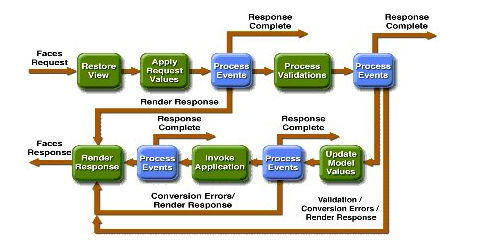
\includegraphics[scale=0.7]{jsflifecycle.jpg} 
\caption{JSF životný cyklus [http://docs.oracle.com/javaee/1.4/tutorial/doc/] }
\label{lifecycle}

\end{center}

\end{figure}
Na obrázku č.\ref{lifecycle} môžme vidieť životný cyklus JSF aplikácie. Počas fázy Restore View, keď je kliknuté na tlačidlo alebo na link sa vytvorí náhľad stránky, spoja sa všetky spracovania udalostí, validátory a komponenty a uložia sa do inštancie FacesContext. V ďalšej fáze Apply Request Values nové hodnoty sú získané použítím metódy decode. Hodnoty sú potom uložené lokálne do komponenty. Pokiaľ nastane chyba, tak je propagovaná a generovaná do FacesContext-u. Na konci tejto fáze sa vykoná znova dekódovanie pokiaľ stály nejaké nové hodnoty vo fronte na spracovanie. Vo fáze Process Validations spracuje všetky registrované validátory ku komponentám. Pokiaľ nastala chyba tak je táto informácia uložená do FacesContext-u. Počas ďalšej fázy Update Model Values nastaví do komponent lokálne nové hodnoty. Počas predposlednej áze Invoke Application je spracované rozličné žiadosti ako potvrdzonie formulára alebo link na iný stránku. V poslednej fáze Render Response dôjde k renderu stránku s novými hodnotami v kotajnery.

\section{Webová služba}
Web Service je sotwarový systém navrhnutý na podporu inteoperability medzi rôznymi zariadeniami prostredníctvom počítačovej siete. Komunikácia prebehia prostredníctvom HTTP protokolu vymenieňaním Extensible Markup language(XML) správ. XML je značkovací jazyk, ktorý definuje sadu pravidiel pre kódovanie dokumentu vo formáte porozumiteľnom človeku prostredníctvom ľubovolných tagov. Webóvé služby poskystujú interoperabilitu medzi rôznymi platformami naprieč počítačou sieťou. Webová služba umožňuje komunikáciu medzi rôznymi aplikáciami, ktoré bežia na rôznych platformách. Tento aspekt je umožnený tým, že aplikácie komunikujú prostredníctov HTTP protokolu. Komunikácia prostredníctvom webovej služby sa delí na 2 učastníkov. Prvý účastník produkovateľ(producer), ktorý vytvára požiadavok a spotrebiteľ(consumer), ktorý prijíma požiadavok. Komunikácia prebieha medzi týmto dvoma učastníkmi výmenov správ. Webová služba môže byť technicky implementovaný rôznymi možnosťami a prostredníctvom Big Web Service alebo Restful WebService, pričom v princípe ako o java triedy, ktoré obsahujú špeciálne definície triedy a metód a pri nasadení na Java EE server môžu byť vzdialenie(po sieti) zavolané ich metódy. 



\subsection{"Big" webová služba}
\uv{Big} webová služba je druh webovej služby, ktorý pre svoju implementáciu používa API JAX-SW\cite{fitWeb} "Big" . Tento typ webovej služby umožňuje vytvárať webové služby orientované na správy alebo techniku vzdialeného volania procedúr(RPC). RPC je technológia, ktorá umožňuje volanie metód, ktoré sa nachádzajú na inom mieste, typicky inom mieste počítačovej siete. Tento typ webovej služby využíva XML správy, spolu so Simple Object Acess Protocol(SOAP) a XML jazykom. SOAP definuje protokol pre výmenu správ založených na jazyku XML prostredníctvom siete prostredníctvom HTTP protokolu. SOAP správy sa skladajú z hlavičky a tela správy, ktoré obsahuje odpoveď webovej služby alebo požiadavok na vyvolanie akcie webovej služby.
\begin{figure}[htb]

\begin{center}

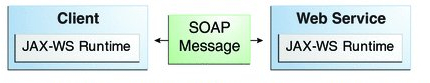
\includegraphics[scale=0.5]{webservice.jpg} 
\caption{\uv{Big} webová služba  prevzaté z [http://docs.oracle.com/javaee/6/tutorial/doc/bnayl.html] }
\label{com}

\end{center}

\end{figure}
Nasledujucí obrázok č. \ref{com} ukazuje spôsob komunikácie medzi klientom, ktorý sa nachádza v ľavej časti obrázku a webovou služba, ktorá sa nachádza vpravej časti obrázku. Komunikácia prebieha prostredníctvom vymienania SOAP správ. Rovnako ako na klientovi tak aj web service obsahuje potrebné API, ktoré spracováva SOAP správy a predáva ich ďalej.

 Tento typ webovej služby obsahuje definíciu vo formáte Web Service Description Language(WSDL). WSDL je definícia vo formáte XML, ktorá popisuje aké akcie webová služba poskytuje a zpôsob ich invokácie, rovnako  aj odpoveď. Správy volania a odpovedí web service sú vymieňané prostredníctvom SOAP správ prostredníctvom HTTP protokolu. JAX-WS API je pomerne komplikované, preto celá komplexnosť je vývojarovi zakrytá a je jediné, čo definuje vývojár sú metódy, ktoré je možné vzdialene volať. Rovnako vývojár nespracováva SOAP správy, ale celá táto problematika je riešená prostredníctvom prostredníctvom API. Veľká výhoda je platformová nezávislosť, ktorá je dosiahnutá prostredníctvom Javy. Tak isto toto API umožňuje prístup k ne-Javovským web service, čo prináša veľkú flexibilitu. Čo sa týka vývoja web service, tak sa jedná o jednoduchú Java triedu, ktorá používa anotáciu javax.jws.WebService, konkrétne anotáciu @WebService, ktorá označuje, že sa jedná o web service endpoint. Táto trieda následne definuje metódy, ktoré môžu byť vzdialené volané. Aby moha byť metóda metódou web service musí byť anotovaná prostredníctvom anotácie  javax.jws.WebMethod @WebMethod. API ponuká aj ďalšie možnosť ako ovplyvňovať životný cyklus web service. 





\section{Princíp webových komponent}
Java EE webové komponenty sú softwarové komponenty, ktoré spracovávajú prichádzajúci HTTP požiadok a poskytujú naň odpoveď. Všetky Java EE webové komponenty sú postavané na servletoch. Servlety sú javovské triedy , ktoré dynamicky spracovávajú požiadavky a tvoria odpovede. Súčasťou servletov alebo webových stránok  sú technológie JavaServer Faces technológiu(JSF) and JavaServer pages(JSP). Servlety podporujú automatickú správu sedenia, prostriedky pre vytváranie a ničenie servletov. Technológie JavaServer Faces a JavaServer Pages podporujú spracovanie užívateľských vstupov a ich predanie a spracovanie podnikovou logikou. Pre implementáciu výslednej aplikáciu bola použitá JavaServer Faces technológia, ktorá poskytuje dostatočné možnosti pri tvorbe webových stránok. V rámci webových komponent spomeniem technológiu, ktorá je potrebná pre pochopenie funkčnosti aplikácie. Ide o technológiu Web Service.



\begin{figure}[htb]

\begin{center}

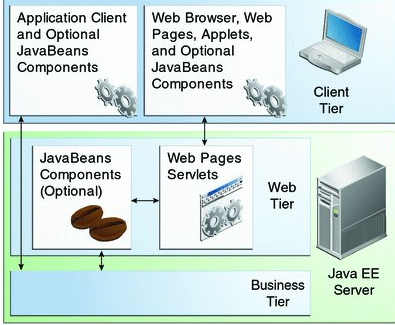
\includegraphics[scale=0.5]{webtechnology.jpg} 
\caption{Webové komponenty [http://docs.oracle.com/javaee/6/tutorial/doc/] }
\label{web}

\end{center}

\end{figure}
Na nasledujúcom obrázku č.\ref{web} je ukázaný princíp fungovania webových komponent. V hornej ľavej časti obrázku sa nachádza klientská vrstva, ktorá obsahuje buď len webový prehliadač po prípade Applety alebo JavaBean komponenty, ktoré čiastočne obsahujú logiku aplikácie. V hornej pravej časti môže byť klient reprezentoný aplikačným klientom, ktorý obsahuje obsahuje úplnú prezentačnú logiku aplikácie a teda v tom prípade, odpadá potreba spracovania vstupov po prípade nejaké generovania html stránky. Takýto klient komunikuje už len priamo s Java EE serverom, konkrétne podnikovým stupňom, ktorý implementuje zvyšnú logiku aplikácie a je reprezentovaný technológiou Enterprise Java Beans. V prípade, že máme k dispozícií tenkého klienta, klient komunikuje prostredníctvom webové prehliadača s HTML alebo XHTML stránky, ktoré sú vytvorené technológiou JavaServer Faces alebo JavaServer Pages, ktoré spracovávajú požiadavok od klienta(vstupy) a následne komunikuje s podnikovým stupňom, ktorý obsahuje logiku reprezentovanú Enterprise Java Beans technológiou, ktorý následne môže komunikovať s databázovým serverom. Odpoveď je následne \uv{predaná} stránkám vytvorené prostredníctvom JavaServer Faces alebo JavaServer Pages technológiou a následne zobrazená užívatelovi v podobe výstupu na webovú stránku. V nasledujúcich dvoch podkapitolách sa bližšie pozreme na technológie JavaServer Faces a JavaServer Pages.




\section{Java Persistence API}
Java Persistence API(JPA) je špecifikácia jazyku Java, ktorá poskytuje prístup, spravovanie dát medzi Java objektmi a triedami a relačnými databázami. Základnou jednotkou JPA je entita, čo je vlastne odľahčený perzistentný doménový objekt, ktorý typicky reprezentuje tabuľku v relačnej databázy a každá jej inštancia je riadkom v  tabuľke. Základný artefaktom v programovaní je pre entity entitná trieda, ktorá obsahuje vlastnosti, ktoré priamo odpovedajú stĺpcov v databáze. Každá entitná trieda priamo musí byť anotovaná javax.persistence.Entity anotáciou. Rovnako musí mať parametrický konštruktor, aby bolo možné vytvárať nové entity. Každá vlastnosť musí pritom spĺňať princíp POJO(Plain Old Java Object), čo znamená, že pre každú metódu musí existovať metóda get a set. Jednotlivé hodnoty môžu byť priamo validované prostredníctvom API JavaBeans Validation prostredníctvom, ktoré je možné definovať anotácie avax.validation.constraints, ktoré definujú aby daná položka spĺňala rôzne vlastnosti(nenulovosť, požiadavky na špeciálny formát vlastnosti, \ldots). Každá entitná trieda má unikátny identifikátor. Týmto identifikátor sa chápe primárny kľúč, ktorý môže byť, môže byť jednoduchý alebo môže byť zložený. Jednoduchý primárny kľúč sa v entitnej triede uvádza prostredníctvom anotácie javax.persistence.Id. V poslednom rade môže byť každá entitna vo vzťahu s inými entitami. Na označenej danej vlastnosti, že sa súčaštou vzťahu s nejakou entitou používame anotácie One-to-one, One-to-many, Many-to-one, Many-to-Many, pričom prostredníctvom anotácie javax.persistence.JoinColumn nám zabezpečuje naviazanie vzťahu s inou entitou. JPA ponúka aj iné, pokročilé možnosti mapovania, pre naše potreby nám budú stačiť nasledujúce informácie. Spravovanie entít je zabezpečované triedou EntityManager, ktorá je reprezentovaná triedou javax.persistence.EntityManager. Každá inštancia tejto triedy je spojená s perzistentný kontextom a určitou množinou entitný tried. Entity manager vytvára a odstraňuje perzistentne entity, umožňuje vyhľadávať entity, rovnako aj vytvárať SQL dotazy nad databázou. Entity manager pracuje s persistencu unit, čo odpovedá definíci entitných tried, s ktorými entity manager pracuje, teda definuje databázové tabuľky, s ktorými entity manager pracuje. Persistence unit sú definované v súbore persistence.xml. JPA rovnako definuje vlastný jazyk Java Persistence Query Language(JPQL), čo je jazyk podobný jazyku SQL, ktorý využíva trieda EntityManager pri svojej práci. Je to jednoduchý reťazcovo založený jazyk na spravovanie entít a vzťahou. Výhodou je, že tento jazyk je nezávislý na zvolenej databázovej technológií a má objektové vlastnosti, teda pri dotazoch nepoužívame konkrétne názvy tabuliek ale názvy entitný tried a jej vlastností. Problém JPQL je typová nebezpečnosť, čo vyžaduje pretypovanie výsledkov dotazu z entity manager-a. To môže spôsobiť chyby, ktoré nemusia byť odchytené počas kompilácie. JPA definuje ešte Criteria API, ktoré je využívané k vytváraniu dotazovou nad entitami a vzťahy, ktoré sú typovo bezpečné. Výhodou tohto API, pre použitie na dotazovanie, je rovnako možnosť vytvárať dynamické dotazy, ktoré majú lepšiu výkonnosť ako JPQL. Pre naše potreby budemé používať obe varianty dotazovania nad dátami v databazy. V poslednom rade treba spomenúť, že JPA je nezávislé nad použitou databázou technológiou, je možné vytvárať dotazy nad MySQL, SQL databázou \ldots. Nakoniec treba zdôrazniť, že JPA nie je konkrétna implementácia ale špecifikácie, implementácie JPA môže byť: Hibernate, TopLink, OpenJPA.


\section{Enterprise JavaBeans}
EnterpriseJavaBeans(EJB) je technológia, ktorá vytvára Enterprise Beans(EB), ktoré predstavujú Java EE komponenty. EJB ďalej predstavuje spravovateľnú, server-side, komponentnú architektúru pre modulárne konštruovanie enterprise aplikácií. Podstatnou úlohou tejto komponenty je zapuzdrenie podnikovej logiky aplikácie. EB pomáha programátorom pri riešení často opakovaných problémov, napríklad perzistencia, bezpečnosť \ldots. V prípade škálovatelnej aplikácie ponúka EB možnosť behu na viacerý zariadenia, rovnako pre väčší počet užívateľov môže existovať viacero EB, ktoré môžu byť rozlične veľké a mať rozličné inštancia v závislosti od požiadavky klienta. EB sa môžu rôzne nachádzať na zariadeniach, ktoré sú prepojené prostredníctvom počítačovej siete a môžu byť volané prostredníctvom štandardného klient/server modelu. Také aplikácie môže byť distribuované a teda poskytovať obsluhu veľkého množstva užívateľov.


EB sa delia na 2 kategórie:
\begin{itemize}
\item Message-driven -  Pôsobí ako poslucháča pre určitý typ správ, ako je API Java Message Service
\item Session - Vykoná úloha pre klienta; voliteľne môže implementovať webové služby

\end{itemize}


\subsection{Session Bean}
Session bean je typ EB, ktorá zapúzdruje podnikovú logiku, ktorá môže byť vyvolaná lokálne, vzdialene alebo prostredníctvom web service klienta.Prístup k session bean sa dejé prostredníctvom volania metód bean-y. Bean-a následne vykoná podnikový kód na serverovej strane. Takýto typ beany nie je perzistentný. Táto beana môže byť ešte 3 typov:
\begin{itemize}
\item Stateful Session Bean - beany udržuje hodnoty premených, každá beana reprezentuje unikátny stav klienta/bean sedenia. Stav komunikácie beany a klienta sa často nazýva \uv{conversational state}, môže mať len 1 klienta, rovnako sedenie môže interagovať len s 1 klientom. Stav je zachovávaný počas klientského/bean sedenia. Pokiaľ sa sedenie odstrániť stav zminzne.
\item Stateless Session Bean - Neudržuje conversational state s klientom. Počas invokácie metódy takejto beany môže inštancia obsahovať premenné, ktoré môžu obsahovať špecifický stav vzhľadom na klienta, alebo len po počas invokácie metódy. Stav beany špecifický pre klienta nepretrváva, ale tento stav môže pretrvať v poll stateless bean počas ďalšej invokáciu metódy. Rovnako jednotlivé inštancie stateless bean sú ekvivalentné takže môžu byť priradené ľúbovoľnému klientovi. Z toho vyplýva, že podporuje viacnásobný prístup klientov a lepšiu škálovatelnosť. Tento typ session beany môže implementovať web service.
\item Singleton Session Bean - Tneto typ beany je inštanciovaný len raz a pretrváva počass celého životného cyklu aplikácie. Využíva sa pri zdieľaní a súčasnom prístupe viacerých užívateľov. Rovnako aj tento typ session beany môže implementovať web service, rovnako udržuje stav medzi invokáciami metód klienta. Tento typ beany môže byť využitý pre špecifické akcie aplikácie, napr. ukončenie aplikácie, štart aplikácie, \ldots, pretože pretrváva počas celého životného cyklu aplikácie.
\end{itemize}

Tento typ beany môžme použiť pokiaľ potrebuje udržať stav medzi klientskými volaniami metód, rovnako pokiaľ potrebuje odľahčiť aplikáciu a zvýšiť výkonnosť použijeme tento typ beany konkrétne stateless session bean. Tieto beany dokážu implementovať web service z tohto dôvodu sme sa rozhodli pre použitie tohto typu EB pre implementáciu web service.

\subsection{Message-driven Bean}
Message-driven bean je typ EB, ktorá umožňuje Java EE aplikáciám asynchronné spracovanie správ. Tento typ beany sa správa rovnako ako Java Message Service(JMS)\cite{messagebook} naslúchavaním správ, ale narozdiel od JMS beana prijíma JMS správy. Tieto správy môžu byť poslané rôznymi Java EE komponentami, alebo JMS aplikáciou alebo aj iným systémom, ktorý nepoužíva Java technológiu. Tieto beany nespracovávajú len JMS správy ale aj iné typy správ. Zásadny rozdiel je medzi message-driven bean a session bean v zásade v tom, že sa k takému to typu beanu nepristupuje prostredníctvom rozhrania a invokácie metód. Tento typ beany obsahuje len bean triedy. Message-driven bean neudržuje dáta alebo conversational state pre klienta. Všetky inštancie takého typu beany sú ekvivalentné, to umožňuje EJB kontaineru priraďovať správy ľubovoľne message-drive bean inštancii. Jedna inštancia beany môže spracováva rozličné správy od klientov. Inštancia premenných môže udržovať stav spracovania klientských správ napr. JMS API connection, databázové pripojenie, \ldots. Klienti pristupujú k message-driven bean, napr. zasielaní správ do cieľa pre message-driven beanu je MessageListener. Message-driven bean má ďalšie zaujímavé vlastnosti a to, že môžu byť vyvolané asychronne, žijú relatívne krátko a sú bezstavové. Pokiaľ správa dorazí do message-driven bean kontajner zavolá metódu onMessage, ktorá pretypuje JMS správy na jeden typ správy a naloží s ňou podľa podnikovej logiky.  Výhodou tejto beany je posielanie asychrónnych správ, ktoré nevyťažujú tak prostriedky servera. Tento typ beany bol použitý pre prijatie požiadavok na spustenie plánovacích úloh a pozastavenie spracovania vzhľadom na možnosť asychrónneho zasielania a zaradzovania požiadavkov do fronty.



\section{Convetion over Configuration}
Convetion over Configuration je sotwarový design, ktoré znižuje počet rozhodnutí, ktoré musí urobiť vývojár a zároveň zvyšuje jednoduchnosť.Po zjednodušení môže tento princíp chápať v zmysle, že vývojár nakonfiguruje len \uv{nezvyklé} aspekty aplikácie. Tento princíp sa snaží odstrániť množstvo konfiguračných súbor, ktoré robia daný projekt neprenositeľný.
Jedným z prostriedkom, ktorý implementuje daný princíp je Maven. Maven je stavebný automatizačný nástroj, ktorý je primárne používaný pre Java projekty. Maven definuje spôsob ako bude sotware zostavený, rovnako aj definuje závislosti(Depency Management). Celý obsah je definovaný v XML súbore, v ktorom sa rovnako definujú závislosti na externé moduly, poradie zostavovania komponent a požadované pluginy. Obsahuje predefinované úlohy ako kompilácia, testovanie, balíkovanie a nasadzovanie. Maven dynimacky sťahuje Javovské knižnice a maven pluginy z jedného alebo viacerých repozitárov ako napr. Maven 2 Central Repository a ukladá ich v lokálnej cache. Maven projekty sú konfigurované prostredníctvom xml súbor, ktorý využíva Project Objec Model a nazýva sa pom.xml, pričom sa nachádza v koreňovom adresári projektu. Nasledujúci obrázok ukazuje štandardnú adresárovú štruktúru maven projektu:

\begin{figure}[htb]

\begin{center}

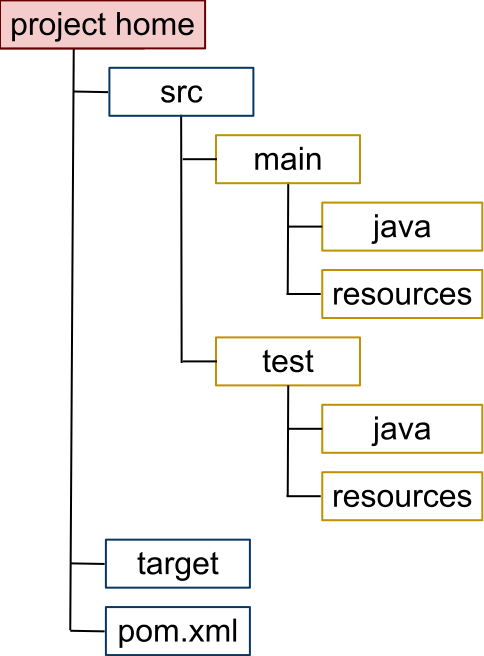
\includegraphics[scale=0.5]{maven.jpg} 
\caption{Maven adresárová štruktúra [http://maven.apache.org/] }
\label{maven}

\end{center}

\end{figure}
obrázok č. \ref{maven} ukazuje základnú adresárovú štruktúru maven projektu. Každý maven projekty sa skladá z project home, ktorý obsahuje súbor pom.xm a všetky ostatné podadresáre. Ďalej sa skladá z priečinkov src, kde sa nachádzajú zdrojové kódy a target, kde sa ukladajú preložené triedy\cite{mavenbook}. Adresár src sa ďalej skladá z adresáru main, ktorý ešte obsahuje adresára java, ktorý obsahuje java zdrojový kód pre daný projekt a resources, ktorý obsahuje prostriedky pre daný projekt ako sú rôzne súbore, ktoré obsahujú nastavenie prostriedkov pre daný projekt. Podadresár src sa skladá z adresára test, ktorý rovnako ako src obsahuje podadresár java, korom je umiestnený java zdrojový kód pre testovanie projektu. Podadresár test obsahuje ďalší adresár resources, ktorý obsahuje prostriedky potrebné pre testovanie. Celá táto štruktúra predstavuje základne adresáru štruktúru pre maven projekt a tak to robí viac prenositeľný. Jednotlivé závislosti pre projekt jednoducho definuje v súbore pom.xml. Preložením projektu sa preložia všetky triedy a uložia do adresára tagert. Celý projekt môže byť pre väčsiu modularitu rozdelený na moduly, pričom každý modul rovnako splňuje základnú Maven adresárovú štruktúru. Každý maven projekt je možné dať ako cieľ jednú z fázy životného cyklu. Životný cyklus môže byť z jednej fáz: 1. validate - validácia korektnosti projektu a kontrola dostupnosti potrebných informácií pre projekt ,2.kompilácia - kompilácia zdrojového kódu projektu, 3.test - testovanie zkompilovaného zdrojového kódu, táto fáza nie je vyžadovaná 4.package - zabalenie zkompilovaného projektu do balíku, napríklad jar, 4. integration-test - spracovanie a nasadenie balíku pokiaľ je to potrebné do prostredia, kde môžu bežať integračné testy, 5.verify-run - beh a overenie balíku, že spĺňa všetky kritéria pre spustenie, 6. install - inštalácia balíku do lokálneho repozitára, v prípade, že potrebuje použiť balík ako závislosť 8.deploy - nasadenie projektu do kontejneru a spustenie.
Jednotlivé fázy môže spustiť príkazom \uv{mvn názov životného cyklu}, napríklad mvn package. Na porovanie výhod Maven som použil nástroj Apache Ant. Ant nástroj nedefinuje presnú adresárovú štruktúru a podporované úlohy narozdiel od maven-u. Definovanie úloh Ant-u sa môžu nachádzať vo viacerých súboroch, pričom každý súbor môže definovať jednu úlohu. Výhodou Ant-u je optimalizácie XML jazyka pre potreby Ant-u pre jasnu definíciu, čo robí a od čoho závisí. Laik je schopný okamžite pochopiť, čo vykonáva xml súbor ant-u.Na druhej strane výhodou Maven-u je, že vývojár, ktorý má skúsenosti s maven-om pochopí okamžite pri neznámom projekte štruktúru projektu a je schopný spustiť štandarné úlohy maven a pozná očakávaný výstup. Z tohto dôvodu som sa pochopil využiť Maven pre svoj projekt, ktorý má rovnako výhodu použítým Depency Management.


\section{Bezpečnosť}
Na zabezpečenie aplikácie bol vybratý framework Seam. Seam je aplikačný framework pre enterprise Javu, ktorý definuje uniformný komponentný model pre podnikovú logiku aplikácie. Takéto komponenty môžu byť stavové, perzistentné a môžu udržovať konverzačný kontext naprieč viacerými webovými žiadosťami. Seam rovnako rieši integráciu EJB a JSF spolu. Rovnako umožňuje písať Seam aplikácie, kde je všetká funkčnosť ukrytá v EJB. Medzi ďalšie výhodné vlastnosti tohto frameworku patrí intergrácia Ajax-u, rovnako aj vstavaná podpora javascriptu a efektívne spracovanie webových dotazov. Seam obsahuje množstvo rôznej inej funkcionality, čím uľahuje písanie enterprise aplikácií, rovnako aj ich udržovanie a efektivity pri vykonávaní definovanej činnosti. My sa zameriame na modul Seam security, ktorý obsahuje množstvo mechanizmov na zabezpečenie našej enterprise aplikácie. Základom každej bezpečnosti je autentifikácia, čo je process vytvorenia alebo potvrdenia identity užívateľa. Užívateľ potvrdzuje svoju identitu prostredníctvom užívateľského meno a hesla, ktoré sa nazýva \uv{credentials}. Seam security poskytuje API prostredníctvom, ktorého je možné sa autentizovať z rozličných zdrojov(databáze, LDAP, \ldots). Ďalšou vlastnosťou je Identity Management, ktoré je množina API na správu užívateľov, skupín a užívateľských rol. Identity Managent je poskytovaný v Seam komponentou PicketLink IDM, ktorá spravuje uloženie užívateľov v rozličných bezpečnostných úložiskách. Poslednými dvoma funkciami tohto modulu frameworku Seam je externá autentifikácia prostredníctvom externých autentifikačných služieb a autorizácia užívateľov na akcie, ktoré môžu v aplikácií vykonávať. Seam security je k dispozícií v prostredníctvom nástroja Maven. Základom authentifikácie je Identity Bean, ktorá reprezentuje identitu užívateľa a pri úspešnej autifikácií je identita je vložená do životného cyklu aktuálneho sedenia. V rámci autentifikácie sú definované metódy Login a Logout. Ďalšou podstatnou časťou je Credentials bean. Táto bean-a udržuje užívateľského informácie(meno,heslo) predtým než sa užívateľ prihlási. Seam secutiry modul poskytuje v rámci autentifikácie rôzne autentifikačné triedy. Základom každej autenfikačnej triedy je metóda autenticate, ktorá autenfikuje užívateľa. Podstatná je metóda setStatus, v ktorej sa nastaví úspech(SUCESS) alebo neúspech(FAILURE) pri overení zadaných údajov. Základom obmedzenia prístupu užívateľov je nainjektovanie triedy Identity, a to môže byť urobené nasledovne, napr. @Inject Identity identity; keď tento kód vložime do managed beany je možné potom v rámci managed beany vytiahnuť informáciu o užívateľovi(užívateľskú rolu, užívateľské meno).
Seam secutiry modul poskytuje spôsob akým zabezpečiť svoje triedy a metódy anotovaním typesafe security binding. Každé typesafe security binding má authorizačnú metódu, ktorá je zodpovedná za to, že určí či užívateľ ma odpovedajúce privilégia k invokácií danej metódy. Základom tvorby typesafe security binding je tvorba rozhrania, napríklad public @interface Admin { }. Následne je potrebné pre dané rozhranie vytvoriť autorizačnú metódu. Autorizačná  metóda je je anotovaná tagom @Secures @Admin(záleží od názvu rozhrania, ktoré môže reprentovať skupinu užívateľov, užívateľskú rolu alebo môže ísť aj o konkrétneho užívateľa). Následne v nej sa overí prostredníctvom Identity triedy, že obsahuje správne údaje alebo mohol byť daný užívateľ priradenený k danému rozhraniu. Tým pádom je umožnený prístup k špecifickým akciám, metódam , \ldots. Pre potreby bezpečnosti bol použitý modul Seam Faces, ktorý je rovnako súčasťou frameworku Seam.Jeho úlohou je integrácia context and depency injection(CDI) do JSF frameworku. Funkčnosť, ktorá nás zaujíma je Faces View Configuration. Ten nám umožňuje spojenie s Seam Security modulom na obmedzenie/povolenie prístupu pre danú užívateľskú rolu, preprepisovanie URL, \ldots. My sa zameriame na povolenie/obmedzenie prístupu k JSF stránkam. JSF stránky sú anotované prostredníctvom vlastností a umiestneé v Java enum-e. Základom je anotovanie rozhrania tagom @ViewConfig a následne tvorba statického enum-u. V ňom sú obsiahnuté anotácie na obmedzenie prístupu k JSF stránkam. Základom je tvorba rozhraní, ktoré obsahujú autorizačné metódy. Následne je možné názvy týchto rozhraní používať k povoleniu prístupu. Pokiaľ máme definované rozhranie Admin(môžeme ho používať anotáciou @Admin) tak pridružením tagu @ViewPattern(), ktorý ódkazuje na nejakú stránku hovoríme, že povolíme užívateľskej role Admin prístup len k stránke definovanej obsahuje tagu @ViewPattern. Takto môže definovať viaceré role. Rovnako môžme definovať ako sa aplikácia zachová v prípade, že úžívateľ sa snaží prístupiť tam, kde nemá prístup. Tento prístup vykonáme použitím tagu @FacesRedirect, ktorý hovorí, že presmeruje @ViewPattern("/*"), teda z ktorej koľvek stránky @AccessDeniedView() na obsahu daný tagom @AccessDeniedView. Týmto zabezpečíme pokiaľ užívateľ z role Admin sa snaží prístupi na stránku, kde má mať prístup len User, tak ho presmeruje na obsah tagu @AcessDeniedView. Seam framework patrí pod divíziu JBoss, takže je pomerne jednoduché ho intergrovať pod aplikačný server JBoss-u. Rovnako je tento framework open-source, čo je jeho ďalšou výhodou.


\section{Testovanie}
V poslednom rade musí technológie, ktoré budem používať pre testovanie. Základom testovania sú 2 technológie, ktoré sme použili jednouchou z nich je technológia JUnit a druhá z nich je technológia Arqullian.
V prvom rade by som sa rád venoval technológií JUnit. JUnit je unit testovací framework pre programovací jazyk Java. JUnit sa používa pre typ testovania, ktorý sa nazýva test-driven development a je jedným z kolekcie unit testovacích frameworkov. JUnit je linkovaný ako jar súbor pri kompilácií a býva súčaštou balíku org.junit. \cite{junitbook}. JUnit testovací inventár je javovský objekt. Testovacie metódy sú anotované prostredníctvom @Test anotácie. JUnit rovnako umožňuje vykonať kód pred spustením testu, to docielime anotovaním metód @Before anotáciou alebo po sputení testu, to docielime anotáciou @After. V testovacej metóde potom vykonáme nejaké kód a očakávaný výstup porovnáme s nami očakávaným výsledok prostredníctvom Assert. JUnit testy sú písané pre otestovanie konkrétnej funkčnosti kódu. Cieľom testovania prostredníctvom JUnit sú malé kúsky kódu, ako metódy alebo triedy. JUnit testy môže použiť rovnako pri písaní kódu alebo pri refaktorizácií na overenie požadovanej funkčnosti kódu. Všetky tieto výhody som využil pri testovaním malých kúskov kódu, ktoré vykonávali požadovanú fukčnosť.

Nakoniec by som rád spomenul technológiu Arquallian. Arquallian je testovací framework, ktorý vykonáva testy vo vnútri vzdialeného alebo vstavaného kontajneru alebo nasadí archív na kontajner, tak aby test mohol interagovať so vzdialeným klientom. Arquallian integruje aj ďalšie testovacie frameworky, napr. JUnit 4, TestNG 5, \ldots, rovnako aj iné frameworky Ant, Maven a iné. Musím zdôrazniť, že narozdiel od JUnit testov umožňuje testovanie v java EE kontajnery(GlassFish, JBoss)\cite{arqbook}. Tento framework má zásadnú výhodu na prenositeľnosť testov na rôzne podporované kotajnery. Testy môžu byť spustené rovnako z IDE tak aj zostavovacím nástrojom. Framework rozširuje aleb integruje existujúce testovacie frameworky. Framework automaticky zabalí do testovacej platformy všetky potrebné prostriedky. V poslednom rade treba spomenúť, že spustenie arquallian testu je veľmi jednoduché. Použitie arquallianu je dané použitím anotácie @RunWith Arquillian, ktoré zabezpečí spustenie testov po spustení. Následne arquallian sputí kontajner nasadí testovací archív, ktorý je daný anotáciou @Deployment. Archív obsahuje testy so špecickými triedami a knižnicami. Testy sa následne vykonajú vo vnútri kotajneru. Čo znamená, že sa použijú všetky dependency a resource inject do testov, takže môžme pristupovať k EJB, rovnako môže pristupovať k databáze, \ldots. Na prvý pohľad vyzeráju arquallian testy ako štandardné JUnit testy. Arquallian umožňuje testovať reálne komponenty, ktoré interagujú s java ee kontajnerom. Arquallian umožňuje spustiť testy vo viacerých módov. Jedným z nich je mód In-cotainer, kde testovanie prebieha priamo v java ee kontajnery pre interakciu s java ee komponentami, druhá možnosť je Client mode, kde testovanie prebieha u klienta u ukazuje ako klient využíva aplikáciu, posledna možnosť je použiť Mixed mode, ktorý kombinuje obe predchádzajúce možnosti. V poslednom rade je potrebné nastaviť kontajner, ktorý sa použije na testovanie. Konfigurácia sa deje prostredníctvom xml súboru arquillian.xml.


\section{JBoss Aplication Server}\label{jbossc}
Aplikačný server(AS) je sotware, ktorý poskytuje vrstvu medzi operačným systémom a java ee aplikáciami. AS poskytuje základnú funkciu programom(prístup k súborovému systému, posielanie správ, \ldots), konkrétne enterprise aplikáciám. Vytvára vrstvu, ktorá zjednodušuje vývoj enterprise aplikácie. Dôvod použitia pre enterprise aplikácie je ten, že tieto aplikácie sú robustné a komplexné a spracovávajú súčasne veľké množstvo požiadavkou od klientov, pričom typickou aplikáciou môže byť webová aplikácia. Pomerne veľká skupina AS je vyvíjaná v jazyku Java. Dôvodom pre tento jazyk existencia štandardu pre enterprise aplikácie a to je Java EE. Nás bude zaujímať implementácia Java EE, ktorá sa nazýva JBoss AS.

JBoss, čo je vlastne skratka pre JavaBeans Open Source Applicatom Server, je aplikačný server, ktorý je založený na platforme Java a Java Enterprise Edition.\cite{jbossbook}. Tento typ AS je open-source, preto je možné jeho stiahnutie spolu so zdrojovými kódmi. Používanie aplikačného servera JBoss je veľmi jednoduché jeho spustenie môžte vykonať ručne prostredníctvom konzole a nájdeným inštalačného adresára JBoss-u a následne adresára bin, ktorý obsahuje skript run.sh, ktorý spustí AS. Druhou možnoštou je spustenie prostredníctvom IDE. Po spustení serveru je možné k nemu implicitne pristupovať na localhost na porte 8080 počítača. Základným stavebným kameňom JBoss AS je JBoss Microcontainer. JBoss Microcontaijner je refaktorizácia JBoss JMX Microkernel aby podporoval POJO nasadzovanie a samostatné použitie mimo aplikačného servera. Microcontainer plní funkciu jadra, do ktorého sa registrujú všetky služby. Služby, ktoré majú by prístupné sa registrujú v podobe managed beans. Microcontainer spravuje a riadi beh týchto služieb. Do AS sa registruje všetko jeho funkcionalita, vrátane Java Management Extention, ktorý umožňuje správu zaregistrovaný služieb. Prostredníctvom tohto rozhranie môžme spravovať všetky zaregistrované služby. JBoss implicitne podporuje databázový server Hypersonic SQL, ktorý má ale obmedzené možnosti, ktorý je určený len na testovanie. Do tohto databázove servera si služby ukladajú informácie.
Tento server je licensovaný pod GNU Lesser General Public License(GNU PL). Dôvod výberu tohto aplikačného servera je integrácia open-source technológií, ktoré sú založené na Jave. Rovnako ako JBoss poskytuje implementáciu širšej škály Java EE technológií, ktoré potrebuje pre vývoj svojej práce. Aplikácie, ktoré bežia na JBoss sú oveľa komplexnejšie.


\chapter{OptaPlanner}\label{optaplannerC}
OptaPlanner je odľahčený open source software a ďalšie prokračovanie frameworku JBoss Drools, ktorý vykonáva a optimalizuje plánovacie problémy. Tento framework je určený pre programovací jazyk java a pomáha programátorom riešiť problémy s obmedzeniami efektívne. Optaplanner kombinuje optimalizačné heuristiky a metaheuristické metódy prostredníctvom kalkulácie skóre. Skóre je hodnota, ktorá reprezentuje bodové hodnotenie riešenia daného problému. Daný plánovací problém môže byť riešený rôznymi optimalizačnými algoritmami. Lepším riešením daného problému je to, ktoré má vyššie skóre. Optaplanner je možné použiť k optimalizácií plánovacích problémov. V bežnom živote, rovnako ako ja v podnikových sférách sa stretávame s rôznymi plánovacími problémami. Môže ísť o problémy ako správne naplánovať cestu vozidiel(aút, lodí,\ldots), aby sme ju spravili za čo najkratší čas, rovnako môžme požadovať aby cesta bola, čo finančne najefektívnejšia. Rovnako môžme plánovanie rozvrhu práce zamestatnancov vo firme, aby zbytočne nespomalovali chod a ostatních zamestatnci, ktorí sú na ich práci závislí nemuseli zbytočne čakať. Plánovať môžme spúšťanie testovania aplikácií v rámci vývojarskej firmy, aby niektoré úlohy boli otestované skôr ako iné no musí byť čo najefektívnejšie vývažené a zbytočne nemrhali časovým kvantom. Plánovacích problémov existuje celá rada a každý deň prichádzame s novými. Pokiaľ je problem dostatočne komplexný potom je veľmi vhodné použiť Optaplanner. Optaplanner môžme používať prostredníctvom maven-u, ktorý poskytuje potrebné triedy na výpočet a konfiguráciu systému, rovnako ako aj nastavenie definičného súboru problému vo formáte xml. Optaplanner je možné použiť aj k riešeniu nedetermisticky polynomiálnych problémov. Na nasledujúcom obrázku môžme vidieť príklad plánovacieho problému

\newpage
\begin{figure}[htb]

\begin{center}

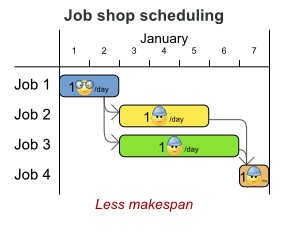
\includegraphics[scale=0.5]{fig/useCaseOverview.jpg} 
\caption{Job, Shop scheluding  [http://www.optaplanner.org/] }
\label{obrazokUseCase}

\end{center}

\end{figure}
Obrázok č. \ref{obrazokUseCase} zobrazuje typické použitie OptaPlanner-u. Môžme vidieť v nasledujúcom obrázku vystupú 4 osoby, ktoré vykonávajú nejakú činnosť. Ich činnosť je špecifická a silne závisí od práce predchádzajúcich. Optaplanner sa snaží ich činnosti maximálne optimalizovať a jednotlivé činnosti zvoliť v následnosti tak, aby výsledná práca bola spravená za najkratší možný čas vzhľadom na činnosť, ktorá sa optimalizuje.


\subsection{Princíp}
Riešenie problému je postavené na práci s definícou problému, ktorý je reprezentovaný xml súborom. Ako sa má daný problém riešiť je dané kódom v Jave. Riešenie je možné ovplyvnoť konfiguráciou Optaplanner-u, v ktorom môžme nastaviť optimalizačné algoritmy plus ďalšie heuristiky, rovnako aj spôsob kalkulácie skóre. Riešenia poskytnutým týmto frameworkom, ktorý využíva pokročilé optimalizačné algoritmy, sú dosiahnuteľné v reálnom čase. Dosiahnutie v reálnom čase znamená nájdenie 1 alebo viacerých riešení, alebo nenájdenie žiadneho riešenia vzhľadom na poskytnutý čas a optimalizačné algoritmy, ktoré sú implementované. Najlepšim riešením je riešenia s najvyšším skóre.



\newpage
\subsection{Ukážka XML configuračného súboru}
V nasledujúcom obrázku by som rád ukázal príklad XML configuračného súboru pre OptaPlanner.
 \lstset{
    language=xml,
    tabsize=3,
    %frame=lines,
    caption=Test,
    label=code:sample,
    frame=shadowbox,
    rulesepcolor=\color{gray},
    xleftmargin=20pt,
    framexleftmargin=15pt,
    keywordstyle=\color{blue}\bf,
    commentstyle=\color{OliveGreen},
    stringstyle=\color{red},
    numbers=left,
    numberstyle=\tiny,
    numbersep=5pt,
    breaklines=true,
    showstringspaces=false,
    basicstyle=\footnotesize,
    emph={food,name,price},emphstyle={\color{magenta}}}
    \lstinputlisting{cloudBalancingSolverConfig.xml}

\newpage
Konfigurácie solveru pozostáva z 3 častí: 
\begin{itemize}
\item Domail model configuration(ja umiestnené medzi tagom <solutionClass>): Definuje hlavnú triedu pre riešenie. Ďalej sa skladá z triedy, ktorá zaobstaráva plánovanie(planningEntityClass).
\item Configurácia skóre, ktorá hovorí Optaplanneru ako ma optimalizovať premenné(tag <scoreDirectorFactory> a podtag <scoreDefinitionType>). Pokiaľ používame hard a soft obmedzenia, použijeme "HardSoftScore". Musíme tiež uviesť ako vypočítať také skóre, v závislosti na našich požiadavkách. Ďalej sa, sme musíme  pozrieť do 2 alternatívy pre výpočet skóre: pomocou jednoduchej implementácie Java(umiestnime triedy to tagu <simpleScoreCalculatorClass>, alebo pomocou Drols DRL(umiestnime do tagy <scoreDrl>.Optaplanner bude hľadať riešenie s najvyšším skóre. Budeme používať HardSoftScore, čo znamená, plánovač bude hľadať riešenie s žiadnymi tvrdými obmedzeniami členenie (spĺňajú požiadavky na hardvér) a pokiaľ možno čo najmenej mäkkých obmedzenia členenie (minimalizovať náklady na údržbu).
\item Konfigurácia optimalizačných algoritmov(tag <constructionHeuristic> a podtag <constructionHeuristicType>). V našom prípade použijeme optimalizačný algoritmus FIRST\_FIT\_DECREASING
\item Voliteľne je možné definovať aj metaheuristiky(umiestnené v tagy <localSearch>). V našom prípade bola použitá metaheuristika TABU SEARCH

\end{itemize}


\subsection{Optimalizačné algoritmy}
V nasledujúcej časti textu si ukážeme optimalizačné algoritmy, ktoré používa optaplanner.
\begin{itemize}
\item First FIT - To je veľmi jednoduché greedy algoritmus aproximácie. Algoritmus spracováva položky v ľubovoľnom poradí. Pre každú položku sa pokúsi umiestniť na položku v prvej priehradke, kde ju môže vložiť. Ak nie je nájdený žiadna priehradka, otvára novú priehradku a kladie položku v rámci nového zásobníka.

\item Firt FIT Decreasing - Tento algoritmus na rozdiel predchádzajúceho funguje nasledovne: Položky sú zoradené podľa ne-rastúcej veľkosti. Ďalším bodom je vždy zabalená položka do prvého koša, kde sa hodí.
\item Firt FIT Decreasing + heurestic local search -  Algoritmus funguje nasledovne: Položky sú zoradené podľa ne-rastúcou veľkosti. Ďalším bodom je vždy zabalené do prvého koša, kde sa hodí. Local search  je metaheuristická metóda pre riešenie výpočtovo zložitých optimalizačných úloh. Miestne vyhľadávanie je možné použiť na problémy, ktoré môžu byť formulované ako hľadanie riešení maximalizuje kritérium medzi niekoľkými kandidátnymi riešeniami. Miestne algoritmy sa pohybujú z roztoku do roztoku v priestore kandidátnych riešení (priestor hľadania) za použitia lokálnych zmien, kým je roztok považovaný za optimálny je nájdený, alebo uplynul čas.

\begin{itemize}
\item Hill Climbing - hill climbing je matematická optimalizácia technika, ktorá patrí do rodiny miestneho vyhľadávania. Jedná sa o iteratívny algoritmus, ktorý začína s ľubovoľným riešenie problému, potom sa pokúsi nájsť lepšie riešenie tým, že postupne mení jeden prvok riešenia. Ak zmena vytvára lepšie riešenie zmeny sa opakujú až žiadne ďalšie zlepšenie nie je možno nájsť.\cite{algobook}




\item Tabu Search - Tabu search používa miestny alebo susedcký postup vyhľadávania tak, že iteratívne presuvá z jedného možného riešenia x k lepšiemu riešeniu x  v susedstve x, kým sa niektoré kritérium zastavenia splní. Miestne postupy vyhľadávania často uviaznu v zle ohodnotených oblastiach. V snahe vyhnúť sa týmto nástrahám a preskúmať oblasti hľadaného miesta, ktoré by mali zostať bez prehliadky inými miestnymi postupmi vyhľadávania, tabu search starostlivo skúma okolí každého toku ako hľadanie postupuje. Riešenie prijatí do novej štvrti sú určené pomocou pamäťových štruktúr.

\item Simulated Annealing - Simulované Annealing je všeobecný algoritmus pre globálne optimalizačné problémy lokalizovať dobré priblíženie k globálnej optimálnej danej funkcie vo veľkom vyhľadávacieho priestoru. To sa často používa pri hľadaní priestorov diskrétnych . U niektorých problémov, môže simulované žíhanie byť účinnejšie ako vyčerpávajúci zoznam - za predpokladu, že cieľom je iba nájsť prijateľne dobré riešenie v stanovenú dobu, skôr ako tým najlepším možným riešením .

\end{itemize}

\end{itemize}






\subsection{Výsledky plánovacieho problému}


Každý plánovací problém je definovaný na základe obmedzení, ktoré musia minimálne spĺnať: \cite{optabook}
\begin{itemize}
\item Negatívne "hard" obmedzenie, ktoré nesmie byť porušené
\item Negatívne "soft" obmedzenie, ktoré by nemali byť porušené pokiaľ sa dá tomu vyhnúť.
\end{itemize}

Niektoré problémy môžu obsahovať aj pozitívne podmienky alebo odmeny, ktoré by mali byť splnené pokiaľ je možné ich splniť.

Tieto podmienky definujú skóre plánovacieho problému. Tieto podmienky môžu byť zapísané v Jave alebo v Drools pravidlách, ktoré značne zjednodušujú kód.

 Vytvorenie pomocou pravidiel  môže robiť  spájanie s inými akciami jednoduchším. Tieto pravidlá bývajú typicky definované pomocou XML súboru.
Optaplanner spajá pri riešení skóre a plánovacie algoritmy.




Bbmedzenia definujú výpočetné skóre problému plánovania. Každé riešenie problému plánovanie môže byť odstupňovaná so skóre. 

Plánovanie problému má niekoľko riešení. Existuje niekoľko kategórií riešení:
\begin{itemize}
\item Možným riešením je nejaké riešenie, či je alebo nie je ľubovoľný počet obmedzení. Problémy plánovania mávajú neuveriteľne veľké množstvo možných riešení. Mnoho z týchto riešení sú bezcenné.
\item Uskutočniteľným riešením je riešenie, ktoré neporušuje žiadne (negatívne)tvrdé obmedzenia. Niekedy nie sú realizovateľné riešenie. Každý uskutočniteľné riešenie je možné riešenie.

\item Optimálnym riešením je riešenie s najvyšším počtom bodov. Problémy plánovanie mávajú jedno alebo niekoľko optimálnych riešení. K dispozícii je vždy aspoň 1 optimálnym riešením, a to aj v prípade , že neexistujú žiadne uskutočniteľné riešenie, a optimálne riešenie nie je možné .
\item Najlepším riešením je nájsť riešenie s najvyšším skóre zistené implementáciou v danom čase.

\end{itemize}

OptaPlanner podporuje niekoľko optimalizačných algoritmov ako efektívne nájsť tieto veľké množstvá riešení. V závislosti na prípade použitia, niektoré optimalizačné algoritmy dosahujú lepšie výsledky ako ostatné, ale to je nemožné povedať dopredu. Pri plánovaní, je ľahké prepnúť algoritmus optimalizácie, zmenou konfigurácie Solver-u.


\newpage


\chapter{Aplikácia}\label{impl}
V tejto kapitole postupne rozobereme problematiku grafického užívateľského rozhrania, použité technológie Rich Faces a Twitter Bootstrap v kombinácií s JavaServer Faces. Výsledné rozhranie bude môcť nahrávať definície problému, zobrazovať výsledky, spúšťať, pozastovať a zobrazovať detaily úloh a nakoniec vyhľadávať úlohy. Keďže táto výsledná aplikácia by mala byť použíteľná aj na mobilnom telefóne bol vybratý štýlovací framework Twitter Bootstrap, ktorý značne uľahčenie tvorbu takéhoto rozhrania. V nasledujúcih kapitolách rozobereme aplikáciu postupne od analýzy až po vyhodnotenie.

\section{Špecifikácia požiadavkov}
Výsledná aplikácia bude zobrazovať priebežné výsledky výpočtu frameworku optaplanner. Tento framework bude pre túto prácu optimalizovaný pre úlohu N Dám, ktorú bude schopný riešiť. Bude sa deliť na aplikáciu, ktorá predstavuje užívateľské rozhranie vytvorené prostredníctvom technológie Java Server Faces v kombinácií s Rich Faces nastylované prostredníctvom frameworku Twitter Boostrap, ktoré zároveň zabezpečuje prenositeľnosť rozhrania na mobilné telefóny. Užívateľské umožňuje zobrazovanie a spravovanie úloh, organizácií, do ktorých náležia jednotliví užívatelia a užívateľov. Každá časť systému bude sprístupnená podľa príslušnosti užívatela k užívateľskej role. Z tohto rozhrania bude môcť užívateľ pokiaľ mu to užívateľská rola dovoľuej pridať úlohu, ktorú môžme následne spustiť alebo pozastaviť. Spustenie prebehia zavolaním služby web service, ktorá obsahuje potrebné prostriedky na spustenie úlohy. Web service následne zavolá enterprise bean, v ktorej prebieha spracovanie danej úlohy. Výsledok výpočtu sa priebežne ukladá do databáze. Výsledku sa následne priebežne zobrazuje v užívateľskom rozhraní. Užívatelia majú prístup k obmedzenému počtu úloh, zároveň môžu vykonávať obmedzené akcie a to nasledovne:
\begin{itemize}
\item Administrátor - má prístup ku všetkým úlohám v systéme, úlohy môže editovať vytvárať, mazať, publikovať a odpublikovať , môže vytvárať, mazať a editovať užívateľov, rovnaké môžnosti má aj s organizáciami
\item Plánovač - má prístup k úlohám v rámci svojej organizácie, môže vytvárať, editovať, mazať úlohy, publikovať a odpublikovať
\item Čitateľ - úlohy môže len zobrať v rámci svojej organizácie, publikovať , odpublikovať
\end{itemize}


Výsledná aplikácia bude nasadená na aplikačný server JBoss.
Nasledujúci obrázok ukazuje príprady užitia systému:
\begin{figure}[htb]

\begin{center}

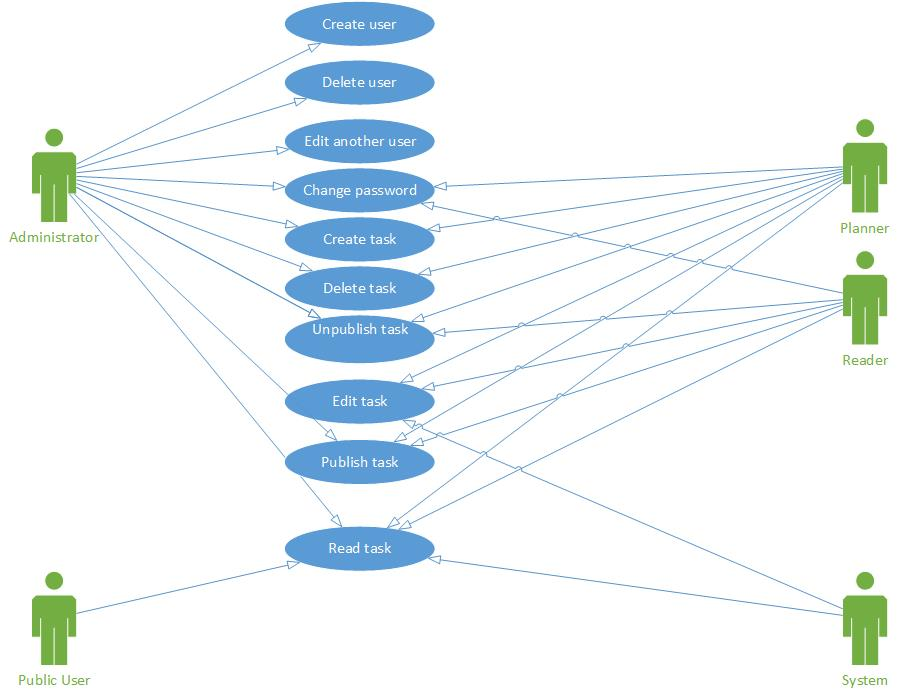
\includegraphics[scale=0.4]{UseCase.jpg} 
\caption{UseCase diagram}
\label{use}

\end{center}

\end{figure}
Na nasledujúcom obrázku č.\ref{use} môžme identifikovať 4 užívateľov systém. Public user je verejný úžívateľ, ktorý môže čítať úlohy, ktoré sú nastavené ako verejné(public) a sú publikované. Systém môže načítať úlohy z databáze pre potreby výpočtu, z ktorými následne pracuje, a potom výsledky ukladá do databáze, teda edituje úlohy(tasky). Čitateľ(Reader) môže úlohy čítať, publikovať a odpublikovať, viac akcií mu nie je umožnené. Plánovač môže úlohy čítať, vytvárať úlohy v databázi, mazať, editovať už vytvorené úlohy v rámci svojej organizácie,publikovať a odpublikovať úlohy a meniť vlastné heslo. Administrátor môže vytvárať úlohy, mazať úlohy , editovať úlohy, publikovať a odpublikovať úlohy. Rovnako si môže meniť heslo, vytvárať,mazať editovať organizácie a rovnaké ackie môže vykonávať pre užívateľov. Zároveň môžu Administrátor, plánovač a čitateľ vyhľadávať v daných úlohách. Administrátor môže následne vyhľadávať užívateľov a organizácie.


\section{Analýza}
Výsledné aplikácia by mohla byť rozdelená na 3 časti. Výsledné rozhranie by mohlo byť vytvorené prostredníctvom technológie Javaserver Faces, ktoré podporuje množstvo komponent na spracovanie a zobrazenie informácií. Pre spracovanie informácií by sme mohli použiť managed beany, rovnako by mohla byť použitá technológia JavaServer Pages, ktorá podporuje skriplety. Druhou časťou aplikácie by bola Web Service rozhranie, ktoré poskytuje metódy na spustenie a pozastavenie úlohy, ktoré bude volané z užívateľského rozhrania. Výpočet by prebiehal v enterprise beane rovnako by bola možnosť výpočet nechať na metódu web service. Rovnako trebalo zvoliť použitú databázovú technológiu existuje veľa možnosti medzi relačnými a nerelačnými technológiami. Medzi 2 zvolené technológie bola relačná technológia MySQL a nerelačná technológia MongoDB. V poslednom rade trebalo zvoliť správny technológiu pre nastylovanie a zabezpečenie prenositelnosť na mobilný telefón. Existuje komplikovaná možnosť  vytvorenia CSS štýlu alebo zvolenia dostupných frameworkov, ktoré túto prácu vyriešia za nás. Jedným z takýchto frameworkov je Twitter Bootstrap. Aplikácia potrebuje pre spracovanie úloh, organizácií a užívateľov databázu. Pre potreby bakalárskej práce bol vybratý relačný open-source databázový model MySQL. MySQL databázová technológia je veľmi vhodná pre malé a stredne veľke aplikácie, čo tá naša je, rovnako poskytuje dobrý výkon pri vykonávaní transakcíí, umožňuje vytvárať procedúry, databázové triggere a jej inštalácia je pomerne jednoduchá a nezaberá veľa diskové priestoru, rovnako je MySQL multiplaformová, keďže je možné ju nasadiť na systémy s operačným systémov windows, linux, max os. Medzi nevýhody tejto technológie patrí neefektívna práca s databázovými transakciami, neefektívne ukladanie veľkého množstva dát. Pre prenositeľnosť na mobilný telefón, rovnako aj pre rýchlu implementáciu riešenia spolu s jeho rozšírením \uv{Awesome Font}. Pre tvorbu rozhrania a spracovanie a zobrazovanie údajov sme použili technológiu JavaServer Faces, ktorá je v porovnnaí s JavaServer Pages oveľa jednoduchšia, keďže použitie skripletov by bolo veľmi komplikované. Z aplikačných serverov bol použitý JBoss, keďže ide o open-srouce riešenie a implementuje plne platformu Java EE narozdiel od Tomcatu, ktorý predstavuje len Java EE servlet kontajner. Aplikácia bola rozdelená na 2 časti rozhranie, web service + enterprise bean-a. Pre bezpečnosť bol zvolený open-srouce framework Seam, konkrétne sme z neho použili moduly Seam Secutiry a Seam Faces. Do úvahy pripadol aj framework OWASP, keďže je Seam súčaštou platformy JBoss, tak sme sa rozhodli pre Seam. Pre implementáciu Web Service bola pouité API JAX-WS, ktoré je oveľa jednoduchšie od JAX-RS. V poslednom ohľade sa uvažovalo o možnosti pravidelné obnovania obsahu tabuľky úloh, ktorá zobrazuje výsledok spracovania úlohy. Pre túto možnosť bola uvažovaná možnosť použitia Ajaxu. Samotné použitie Ajaxu v JSF aplikácií zbytočne komplikované, preto bola zvolená možnosť použitia Rich Faces, ktorý podporuje Ajax komponenty a poskytuje jednoduchú integráciu s JSF aplikáciou.


Tento typ BIGFULL WEB SERVICES technológie bol zvolený z dôvodu potreby komunikácie užívateľského rozhrania so systémom na výpočet, ktorý sa nachadzá na inom výpočetom zariadení a tieto zariadenia si vymieňajú informáciu prostredníctvom HTTP protokolu. Umožňuje nám teda zdieľať funkčnosť kódu prostredníctvom siete a jej vzdialené volanie. Ďalšou výodou tejto technológie využívajú štandardizované protokoly komunikácie, čo umožňuje jednoduchú interoperability medzi inými systémami. Keďže táto technológia používa pre komunikáciu HTTP protokol využíva pre komunikuje prostredníctvom štandardnej počítačovej siete, čo žnižuje náklady na prevádzkovanie na rozdiel od iných proprietárnych technológií.

Dôvod vybratia tohto druhy web service je ten, pretože umožňuje využívať mechanizmy pre QoS a poskytuje štandardy na zabezpečenie spoľahlivosti.


\subsubsection{Twitter Bootstrap}
Twitter Bootstrapje veľmi jednoduchý a voľne dostupný súbor nástrojov pre vytváranie moderného webu a webových aplikácií.\cite{boot} Ponúka podporu najrôznejších webových technológií HTML , CSS , JavaScript a mnoho prvkov , ktoré je možné ľahko implementovať do svojej stránky. Pre použitie Twitter Bootstrap sú nutné základné znalosti HTML a CSS. Interaktívne prvky ako sú tlačidlá, boxy , menu a ďalšie kompletne nastavené a graficky spracované elementy je možné vložiť iba pomocou HTML a CSS .

Výhodou tohto súboru nástrojov je jednoduché spracovanie akéhokoľvek používateľského rozhrania vo webovej aplikácii a nerozhoduje , či to je napríklad používateľské rozhranie v administrácii back-endových alebo front-endových aplikácií. Tak isto podporuje zobrazenie aj na mobilných telefónoch.


Podrobné vysvetlenie jednotlivých komponent nájdete na nasledujúcej adrese http://getbootstrap.com/, rovnako aj s príkladmi použitia. Výhodou a dôvodom použitia tohto frameworku je lahká integrácia do webovej aplikácie, rovnako aj open source charakter a v poslednom rade množstvo príkladom použitia. V poslednom rade bolo použité rožšírenie Font Awesome, ktoré obsahuje framework, ktorý obsahuje ikonové fonty určené pre twitter boostrap.


\subsubsection{Rich Faces}
Rich faces predstavuje open-source Ajax knižnicu, ktorá predstavuje rozšírenie pre JavaServer Faces. Umožňuje integráciu schopností ajaxu do enterprise aplikácií. RichFaces obohacuje framework Ajax4jsf v dvoch dôležitých ohľadoch. Po prvé, sa rozširuje množstvo vizuálnych pripravených komponent. Po druhé,  plne implementuje funkciu skinnability rámca Ajax4jsf vrátane veľkého množstva preddefinovaných vzhľadov. Pomocou skinnability, že je oveľa ľahšie riadiť vzhľad aplikácie. Jej zásadnou a už spomenutou výhodou je implementácie množstvo ajax komponent, ktoré sa jednoducho používajú a integrujú do JSF aplikácie. Použitie tohot frameworku je možné prostredníctvom maven-u.





\section{Návrh aplikácie}
Aplikácia bola rozdelená na 2 časti. Jednou častou je samotné grafické užívateľské vytvorené technológiou JSF skombinované s rôznymi frameworkami. Táto aplikácia komunikuje s databázou prostredníctvom JPA s databázou technológiou MySQL. Rovnako zobrazuje informácie úlohách a ďalšie informácie podľa užívateľskej role, rovnako spracováva vstupy zadané užívateľov. Spustenie a zastevenie úloh je vykonáva prostredníctvom Message-driven beany. Signál daný message-driven beany je daný cez web service, ktorá dostane požiadavku od JSF aplikácie. Tá následné predá požiadavok message-driven beane. Požiadavky sa radia do activemsq fronty. Z tejto fronty sú postupne odoberané požiadavky message-driven beanami, ktorá spustia plánovanie(výpočet úlohy). Do fronty sú umiestňované ID úlohy, ktoré sa majú spustiť. Výpočet potom prebieha vytiahnutím xml súboru a spustenie výpočtu, pričom sa priebežne ukladajú informácie o skončení úlohy, rovnako aj informácie percentuálnom pokroku úlohy. Po skončení úlohy sa zmení stav úlohy a uložia sa informácie o dokončení úlohy. JSF aplikácia každých 4 sekúnd aktualizuje stav úloh z databáz a zobrazuje ich užívateľovi v prehliadači. Úlohu je možné aj pozastaviť. 





\subsection{Návrh modelu databáze}
Na nasledujúcom obrázku je ukázaný ER diagram, ktorý bol použitý pre dtabázu:
\begin{figure}[htb]

\begin{center}

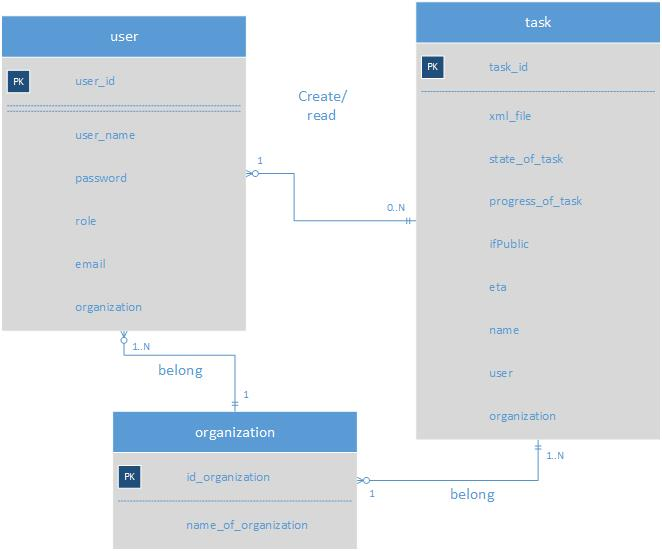
\includegraphics[scale=0.5]{ER.jpg} 
\caption{ER diagram}
\label{ER}

\end{center}

\end{figure}

Tento obrázok zobrazuje jednotlivé entity, ktoré sú potrebné na uloženie v databáze, každá z nich ma určité položky. ER diagrama sa skladá z 3 entít: user - entita, ktorá reprezentuje užívateľ, task - entita, ktorá reprezentuje úlohu a organization - entita, ktorá reprezentuje organizáciu. Výsledný návrh odpovedá skutočnosti, že každý užívateľ musí byť súčašťou organizácia, rovnako môže mať vytvorené 0 až N úloh. Taktiež pre zjednodušenie je každa úloha priradená priamo organizácií pre zlepšenie rýchlosti získania výsledkou a zjednodušenia ich nájdenia. Každá entita obsahuje primárny kľúč(jedná sa o silné entitné množiny), ktorý je odvodený od názvu a začína predponou \uv{id\_} a pokračuje názvom entity s Camel notáciou. Poďme sa pozrieť bližšie na jednotlivé entity. Entitná množina organization obsahuje 2 položky jednou z nich je primárny klúč a ďalšou názov organizácia podľa, ktorej sú zaraďovaný jednotlivý užívatelia. Ďalej prejdime k entitnej množine user. Táto entita má rovnako primárny kľúč. Ďalej obsahuje položku pre užívateľské meno(username), heslo(password), email, užívateľskú rolu(role) a cudzí kľúcč organization, ktorý obsahuje na organizáciu. Nakoniec prejdime k entitnej množine task. Táto entitná množina obsahuje primárny kľúč, ďalej obsahuje xml súbor, ktorý reprezentuje danú úlohu(v našom prípade N dám), stav úloh(stateOfTask, ktorý reprezentuje rôzne stavy úlohy), ktorý si podrobnejšie rozobereme. Úloha sa môže nachádzať v jednom z nasledujúcich stavov:
\begin{itemize}
\item NEW - úloha bola vytvorená
\item MODIFIED - xml súbor bol modifikovaný
\item WAITING - úloha čaká na spracovanie
\item IN\_PROGRESS - práve prebieha výpočet
\item PAUSED - úloha je pozastavená
\item COMPLETE - úloha je dokončená
\end{itemize}
Entitná množina task ďalej obsahuje položku, ktorá percentuálne hodnotí stav výpočtu úlohy(progressOfTask), čas do skončenia výpočtu úlohy(eta), nastavenie úlohy na privátnu alebo verejnú(ifPublic), názov úlohy(name) a cudzie kľúce user, ktorý odkazuje na užívateľa, ktorým bola úloha vytvorená a organization, ktorá odkazuje na organizáciu užívateľa, ktorým bola vytvorená. V ďalšej kapitole sa pozrieme na use case diagram.

\subsection{Návrh užívateľského rozhrania}
Výsledné rozhranie kladie dôraz na jednoduchosť a prehľadnosť zobrazených úloh. Z tôhto dôvodu boli implementované mechanizmy vyhľadávanie úloh, organizácií a užívateľov. Rovnako možnosti lexikografického triedenia. Po prihlásení do systému Jednotlivé môžnosti sú následe zakompotované do záložiek, v ktorých je sprístupné príslušná funkčnosť. Výsledné rozhranie je prenositeľné aj na mobilné zaradenie, čo je spôsobené použitím frameworku Twitter Boostrap. Je ešte lepšiu prívetivosť bolo použité rozšírenie Font Awesome. Užívateľské rozhranie je popísané na nasledujúcom obrázku:
\begin{figure}[htb]

\begin{center}

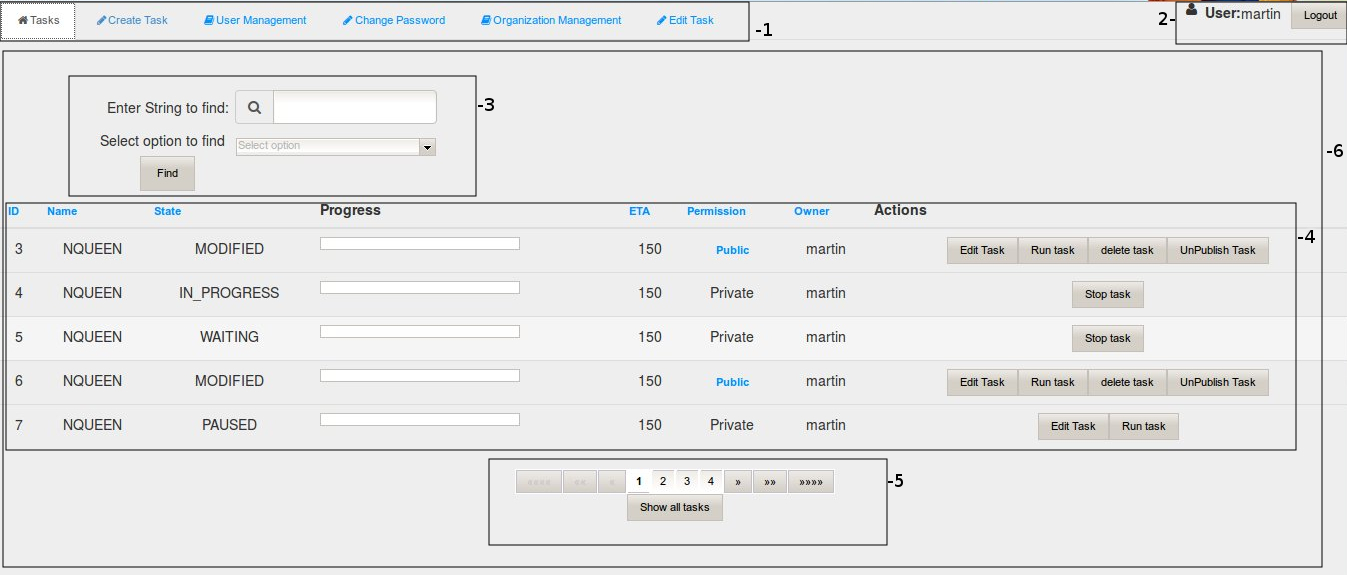
\includegraphics[scale=0.5]{page_show.jpg} 
\caption{Návrh užívateľského rozhrania}
\label{rozhranie}

\end{center}

\end{figure}
Na obrázku č.\ref{rozhranie} môžme vidieť návrh užívateľského rozhrania. Rozhranie je rozdelené do 6 častí, ktoré môžme rozoznať na obrázku číslami od 1 do 6, ktoré sú aj ohraničené. Celé rozhranie môžme rozdeliť do nasledujúcich častí:
\begin{itemize}
\item Oblasť č.1 predstavuje navigačné menu, kde sú jednotlivé akcie rozdelené do záložiek podľa ich názvu. Pre klinutí na príslušnú záložku sa zmení aj obsah na stránke. 
\item Oblasť č.2 obsahuje informáciu o prihlásenom užívateľovi , rovnako obsahuje aj tlačidlo \uv{Logout}, prostredníctvom ktorého sa môže užívateľ z aplikácie odhlásiť
\item Oblasť č.6 predstavuje funkčnú oblasť. Táto oblasť je špecifická pre každú záložka, ktorá reprezentuje jej obsah. V tej oblasti sú umiestnené typicky obsahy databázových tabuliek, nástroje na vyhľadávanie, rôzne akcie, ktoré je možné vykonávať s dátami, rovnako aj možnosti na vytváranie entít
\item Oblasť č.3 predstavuje jednu z funkčných možností. Jedná sa o vyhľadávanie, ktoré je zložené zo vstupného prvky, do ktorého zadamé vyhľadávaný reťazec a druhá časť predstavuje menu,z ktorého zvolíme stĺpec na vyhľadávanie. Následne je možnosť realizovať tlačidlom Find, ktoré prekreslí obsah tabulky nižšie a naplní ju nájdenými výsledkami.
\item Oblasť č.4 predstavuje tabulky, ktorá je dynamicky obnovaná a reaguje na asychronné ukladanie dát z web service, ktoré sa dynamicky obnovujú každé 4 sekundy. Tabuľka je rozdelená do stĺpcov. Názvy stĺpcov, ktoré sú označené modrou farbou sú zároveň odkazy, na ktoré je možné klinúť. Po kliknutí na daný odkaz dôjde k lexikografickému zoradeniu obsahu tabuľky podla daného stĺpca striedavo vzostupne alebo zostupne. Rád by som upozornil na stĺpec progress, ktorý pre každú úlohu zobrazuje stav spracovania úlohy. Rovnako musím zdôrazniť stĺpec Permission, ktorý zobrazuje, či je úloha verejná alebo privátna. Pokiaľ je úloha verejná(Public), tak je tento odkaz zobrazený modrou farbou, čo znamená, že je odkaz preto je možné naň ho kliknúť. Po kliknutí sa zobrazí stránka s informáciami o názve úlohy a obsahuje výsledného xml súboru. Tento odkaz je možné následne ľubovolne preposlať a pristupovať k nemu. V poslednom rade treba zdôrazniť stĺpec \uv{Actions}, ktorý je najdôležitejší pre každú úlohu povoluje sadu akcií. Jednotlivé akcie sú reprezentované tlačidlami, pritom odrážajú aktuálny stav spracovania úlohy spolu s ďalšími informácimi o úlohe.
\item Oblasť č.5 predstavuje komponentu na stránkovanie, aby pri rozsiahlom obsahu sa nezväčšoval neúmerne veľkosť stránky.


\end{itemize}

Zvyšné návrhy rozhrania je možné dohľadať v prílohe.






\section{Implementácie}
Aplikácie bola rozložená do viacerých tried podľa zodpovednosti daných komponent. Pri implementácií bolo použité JBoss Developer studo 7.1.1 GA spolu s JBoss AS 7.1.1 Final. Celý projekt boli založený na technológií maven, ktorú uľahčovala celý process vývoja a jeho následne nasadenie na JBoss server. Pre databázovú technológiu bol nainštalovaný mysql server nakonfigurovaný s príslušnými údajmi.

\subsection{Rozdelenie aplikácie}

	Aplikácia bola rozdelená na 2 časti:
	\begin{itemize}
	\item JSF aplikácia s užívateľským rozhraním, ktorá zobrazuje výsledky, umožňuje spravovanie databáze, rovnako aj pristupovanie k službám web service, je pritom rozdelená na hlavný modul s celou funkčnosťou a modul s entitami, ktoré zdieľa s PlannerService - optaplanner.controller
	\item Web service + EJB aplikácia, ktorá poskytuje web service koncový bod spolu s metódami na spustenie a pozastavanie úlohy. Spustenie úlohy volá Message-driven Beanu, ktorá vykonáva spravanie(plánovanie) úlohy, využíva pritom modul Enties, ktorý obsahuje entitné triedy - PlannerService

	\end{itemize}




\subsection{JSF aplikácia}
JSF aplikácia bola postavená na technológií JavaServer Faces v kombinácií s frameworkami Rich Faces, Twitter Boostrap a Font Awesome.  Aplikácia zabezpečuje prihlasovanie užívateľov v kombinácií s bezpečnosťou, ktorá je implementovaná s frameworkom Seam. Je rozdelená na .xhtml stŕanky podľa užívateľskej role. Na každej stránke pritom môžme nájsť komponenty, ktoré dovoluju užívateľovi príslušné akcie. Na .xhtml stránkach sa následne zobrazuje aj obsah spracovania, ktorý už bol prezentovaný tak aj entity užívateľov a organizácií spolu s ich spravovaním. Tieto komunikujú prostredníctvom expression language s managed beananmi na pozadí, ktoré rovnako vykonávajú aj validáciu jednotlivých komponent(od nepovolených hodnot, až po prázdne vstupné polia). Stlačenie príslušného tlačidla spôsoby zavolanie metódy z managed beany a vykonanie akcie, pričom jej obsah môže byť ale nemusí byť zobrazený na .xhtml stránku.
	

\subsection{Prihlasovanie}
Prihlasovanie je realizované prostredníctvom frameworku Seam, z ktorého sme využili moduly Seam Faces a Seam Security. Pre každú užívateľskú roli bolo vytvorené rozhranie a metódy, ktoré overovali indentity užívateľa. Pre prístup musela mať užívateľ danú užívateľskú rolu, pričom prístup bol implementovaný enum-om, v ktorom kažej role, ktorá bola reprezentovaná anotáciou(@Administrator,@Reader, @Planner) boli povolené len im prislúchajúce stránky a bolo deklarované, čo sa má vykonať pri po pokuse o nepovolený prístup(presmerovanie na prihlasovací formulár). Prihlasovanie rovnako obsahovalo validáciu a informovalo užívateľa o nevalidnom hesle, alebo mene. Po úspešnom prihlásení bola do životného cyklu vložená Identita a užívateľ bol presmerovaný na jemu prislúchajúcu stránku. Vloženie identity malu tú výhodu, že bolo možné z managed beany zistiť aký je prihlásený užívateľ. Prihlasovanie overovalo údaje z databáze, pričom pre overenie hesla používalo tŕiedy ShaEncoder, ktorá obsahuje hash funkcia prostredníctvom, ktorej sú zabezpečené všetky heslá v databáze.

\subsection{Logika JSF aplikácie}
V prvom rade trebalo správne nakonfigurovať súbor persistence.xml, aby ukazoval na nami definovaný datasource v rámci aplikačného servera. To umožňuje pristupovanie k dátam v databáze.
Celá logika aplikácie bola sústredná bola sústredená do managead bean, pričom 1 managed beana podľa prihláseného užívateľa(napr. užívatelská rola administrátor na stránke Administrátor.xhtml bola spravovaná managed beanov AdministratorBean). Tie obsahovali metódy a vlastnosti, ktoré bola zobrazované/prevzaté z komponent na .xhtml stránke. Vlasnosti museli spĺňať princíp POJO. Metódy následne volali podľa potreby databázové operácie, ktoré boli sústredené v balíku databaseOP v triede Operation. Tá obsahovala metódy na mazanie, update, vytváranie entít. Predpisy entitných tried sa nachádzali v module Entites. V balíku service sa nachádzali triedy, ktoré umožňujú volanie metód web service.

\subsection{Implementácia rozhrania}
Pre implementáciu rozhrania som využil technológiu xhtml stránok. Pre každú užívateľskú rolu som vytvoril xhtml stránku identitickú s názvom užívateľskej role. Pre prihlasovanie bola použitá Login.xhtml stránka. Na Login.xhtml boli umiestnené komponenty na zadanie užívateľského mena a hesla vrátane skrytých validačných komponent. Pre implementáciu xhtml pre užívateľské role sa zameriam na užívateĽskú rolu Administrátor, keďže rola Plánovač a Čitateľ prevzali všetku implementáciu a komponenty práve od Administrátor, ale len v obmedzenom množstve, teda komponenty vrátane akcií, ktoré mohli vykonávať. XHTML stránka sa skladá v hornej časti z menu, ktoré je implementované ako záložky prostredníctvom Twitter Boostrap-u. V pravej hornej časti sa nachádza informácia o prihlásenom užívatelovi vrátane tlačidla na odhlásnie. Pri kliknutí na záložky sa zobrazí obsah, ktorý odpovedá názvu záložku. Záložky \uv{user management, task, organization management} obsahujú komponenty h:datatable z knižnice JSF pre zobrazenie dát. Tieto dáta sú pravidelné obnovované komponentov z knižnice Rich Faces a4j:poll, ktorý využíva Ajax pre obnovenie obsahu. Každá z tých záložiek obsahuje pole pre vyhľadávanie pričom je možné zvoliť podľa, ktorého stĺpca sa bude vyhľadávať. Výsledky sa zobrazia do tabuľky(h:datatable) pričom zobrazené položky budú odpovedať nájdeným výsledkom. Pri každej položke v tabuľke je možné vykonávať isté akcie ako je vymazať danú entitu, po prípade ju editovať, alebo vykonávať množstvo iných akcií. Akcie pritom reflektujú individuálny stav danej entity.Pri každej z tých záložiek okrem task(ktorú v zápäti rozoberem) je možné entity aj vytvárať. Vytváranie je veľmi jednoduché, keď užívateľ vyplní všetky polia, ktoré musí mať daná entita. Každú tabuľke je možné aj radiť. Radenie prebieha kliknutím na názov stĺpca tabuľky, pričom danú stĺpec implementuje funkciu radenia pre daný stĺpec len v prípade, že názov je vyznačený modrou farbou. Vytváranie úloh(taskov) je zaradené do samostatnej záložky kvôli lepšej prehľadnosti. Užívateľ vyplní meno a prostredníctvom komponenty na nahrávanie súboru z knižnice Rich Faces nahrá obsah do databáze. Ďalej rozoberem záložku change password, ktorá umožňuje si pre daného užívateľa zmeniť heslo, vyplní pritom heslo a potvrdenie heslo a heslo sa zmení. Nakoniec rozoberem záložku edittask, táto záložka je pri bežnom prehliadaní prázna je to spravené kvôli bezpečnosti. Táto záložka sa aktivuje editovaním úlohy v záložke task, ktorá nás prepne do záložky edittask, v ktorej sa už aktivuje obsah a užívateľ vyplní názov úlohy,vlastníka úlohy a nakoniec edituje xml súbor úlohy. Potvrdením sa vytvorí úloha so stavom "MODIFIED".





\subsection{Web Service, EJB aplikácia}
Pri implementácií web service bola využitá už čiastočne implementovaná Web service, do ktorej boli následne doplnená funkčnosť spustenia úlohy a pozastavenia úlohy. Jej časť spustenia výpočtu už nebola cieľom bakalárskej práce a bola teda implementovaná mojim vedúcim Martinom Večeřom.
Táto aplikácia je pomenovaná PlannerService a obsahuje ako som spomínal Big Web servica s 2 metódami. Tieto métody sú metóda runTask s jedným parametrom a to ID úlohy, ktorá sa má spustiť. Pričom dôjde k vytvoreniu spojenia s Message-driven bean,ktorá vykonáva výpočet. Najprv sa do fronty zaradí ID úlohy, ktorá sa má spustiť. Následne si Mesage-driven beana získa z fronty ID úlohy a následne spustí výpočet. Tieto beany sa kvôli rozloženiu záťaže môžu nachádzať na viacerých serveroch. Priebežne pritom aktualizuje stav spracovania úlohy. Priebežne pritom ukladajú údaje o stavu úlohy, času do ukončenia úlohy a percentuálnom ohodnotení úlohy. Po ukončení úlohy je uložené najlepšie možné riešenie do databáze. Na skončení spracovania nastaví príslušný stav úlohy a skončí. Web service obsahuje aj metódu na pozastavenie výpočtu s 1 parametrom a to je ID úlohy, ktoré sa má pozastaviť. Tá následne zavolá Message-driven bean-u, ktorá si z fronty získa úlohu a pozastaví jej výpočet. Tie si úlohu vyberú z actiemsq fronty a spustia výpočet. 
	
	



 
\section{Testovanie}
Testovanie prebiehalo na servery JBoss AS 7.1.1 Final najprv prostredníctvom jednodúch JUnit testov, ktoré malo overiť komplikovanú fukčnosť metód. Následne sa pre overenie fukčnosti databáze použil framework Arqullian, ktorý umožňuje nasadenie tried priamo do Java EE kontajneru, čo zjednodušuje testovanie. Prostredníctvom tohto frameworku sa testovala celková fukčnosť aplikácie. Jednoduchšie časti boli otestované pomocou JUnit testov. Postupným budovaním aplikácie sa pristupovalo k testovaniu navrhnutých častí. Junit boli postupne skonštruované pre jednoduchšie metódy, ako je overenie funkčnosti vyhľadávania entít, mazanie entít, pridanie entít do zoznamu úloh. Pomocou arquallian-u bolo následné otestovaná prihlasovanie, databázové operácie, rovnako bola otestovaná bezpečnosť aplikácie.


V ďalšej častie prebiehalo testovanie medzi konkrétnymi užívateľmi. Užívatelia testovali aplikáciu a hľadali buggy, ktoré neodhalilo predošlé testovanie. Rovnako overovali, či boli splnené formálne požiadavky. Skupine užívateľov bol predložený odkaz na nasadenú aplikáciu a prihlasovacie údaje. Užívatelia mohli následne sa prihlasovať pod rôznymi užívateľskými rolami, tí nasledne testovali vytváranie užívatelov, organizácií, úloh. Následne mohli sledovať stav spracovania plánovacich úloh. Aplikáciu otestovali pod 2 prehliadačmi a to Google Chrome vo verzii 34.0 a Mozilla Firefox verzie 28.0. Bol použitý operačný systém linux 3.13.0-24-generic s operačným systémom Kubuntu 14.04.Aplikácia sa správala pod obomi rovnako a korektne. Po odhalení chýb boli chyby ohlásené a odstránené a aplikácia bola následne opäť nasadená. Tento postup sa opakoval až dokým neboli odhalené všetky chyby. 




\section{Vyhodnotenie aplikácie}
Po testovacej fáze nasledovala fáza vyhodnotenia aplikácie. Cieľovej skupine bol po opravení chýb aplikácie predložený dotazník, do ktoréh výplňami rôzne informácie, kde dávali spätnú väzby, chyby v návrhu, rovnako aj v intuitívnosti ovládania. Cieľovou skupinou bolo 7 eventuálnych používateľov tejto aplikácie. Z dotazníka nám vyplynuli nasledujúce názory a pohľady na aplikáciu.


















\chapter{Záver}\label{zaver}
Plánovanie s ním spojené problémy narážame v bežnom živote čoraz častejšia. Ešte väčšie problémy tohto typu majú organizácie, ktoré musia dennodenne riešiť ako naplánovať efektívnu prácu svojich zamestnancov, ako správne komunikovať so zákazníkom a mnoho iných problémov. Riešenie klasickým prístupom a to využitím ľudskými zdrojmi je časovo neefektívne, rovnako treba brať do úvahy ľudský faktor. Preto vzniklo riešenie, ktoré odbremeňuje organizácie od riešení komplikovaých plánovacích úloh. Taký software je šírený pod licenciou open-source a nazýva sa Optaplanner. Tento systém je následne možné využívať pre akúkoľvek oblasť plánovania, aká len nás napadne. Jediné obmedzenie tohto systému sú použité plánovacie algoritmy kobinovaný s rôznymi heurestikami. Užívateľ je schopný definovať definíciu problému, pričom sa môžme inšpirovať verejne dostupnými príkladmi, vytvoriť si pravidlá a nechať systém nech nájde optimálne riešenie pre daný problém. Vytvorená aplikácia predstavuje jedným zo spôsobov ako daný systém využiť pre plánovanie. Aplikácia je intuitívna, formálne spĺňa požiadavky, rovnako sú predstavené možnosti rožširenia rozhrania a urobenie tohto rozhrania oveľa užívateľsky prívetivejšie.  Rovnako ukazuje akým spôsobom bol systém navrhnutý z implementačného hľadiska, sú vysvetlené technológie potrebné pre implementácui so zreteľom na výhody použitia. Pre systém bol použitý aplikačný server JBoss, ktorý predstavoval medzi dostupnými riešenia najlepší java EE kontajner. Pre lepší návrh by mohla byť aplikácia rozšírená na použitie ich iných plánovacích úloh, rovnako môže byť užívateľské rozhranie rozdelené do viacerých samostatných sekcií kvôli lepšej prehľadnosti. V poslednom rade kvôli lepšej pochopiteľnosti aplikácie by mohla byť JSF aplikácia rozdelená do viacerých balíkov.


